\chapter{Research Context}%
\label{chap:research_context}

Highly automated driving is currently an immensely attractive field for both academic and industrial research groups.
A fully autonomous vehicle, which is able to tackle challenging driving situations without external input comparable to a human driver's performance, is yet to be build.
In this thesis, we propose a novel approach to knowledge and information representation for automotive environment models using cognitive modeling techniques.
More precisely, we adopt \acfp{VSA}, which are commonly used in tasks like cognitive modeling and natural language processing, for the specific application of automotive environment modeling.
To our knowledge, \acp{VSA} have not been applied in this particular context.
In order to put our work in context of the current research landscape and to circumscribe this thesis, we need to review related work from several areas like automated driving and mobile robotics, computational neuroscience, artificial intelligence and neuromorphic engineering.
A comprehensive overview for all of these research areas is out of scope of a single thesis.
However, we aim to cover the most significant results from all areas at least briefly, whereas we present an in-depth review of relevant work related to the thesis at hand, where necessary.

\section{Biologically-inspired Systems}
\label{sec:bio_systems}

To fully understand biological systems like the brain, which evolved over millions of years, is an ongoing yet unsolved challenge in biology and neuroscience.
Even small animals like insects or rodents show remarkable behavioral flexibility and the ability to constantly adapt to a rapidly changing and noisy world, which is unmatched by modern computing machines.
Mammals and primates are able to perform more sophisticated behaviors culminating in complex cognitive computations humans are capable of doing like thinking, problem solving, memory, reasoning, decision-making, strategic planning, knowledge representation, learning etc.
The "biological computer" enabling these behaviors and cognitive abilities is the brain consisting of large networks of neural cells (or neurons), which communicate by sending and receiving electric signals via synapses.
At the same time, brains are comparably small and efficient: the human brain for example consumes only \SI{20}{\watt} of power (equivalent to a compact fluorescent light bulb) and comprises \SI{2}{\percent} of the body weight \cite[Chap. 2.1]{Eliasmith2013}. 

Several research fields like computational neuroscience, neuromorphic engineering and neurorobotics try to reverse engineer biological systems to achieve similar performance and computational power.
During the last decades, researchers and engineers strived to close the gap in performance and efficiency between biological and artificial computing systems by mimicking neuro-biological architectures in hardware and implementing models of neural systems in software.
This biologically inspired, \textit{neuromorphic} approach promises not only to perform computations in a more efficient way, but also to tackle problems unsolvable with current computing machines.

\subsection{A brief history}%
\label{subsec:history_neural_nets}

\begin{figure*}[t!]
	\centering
	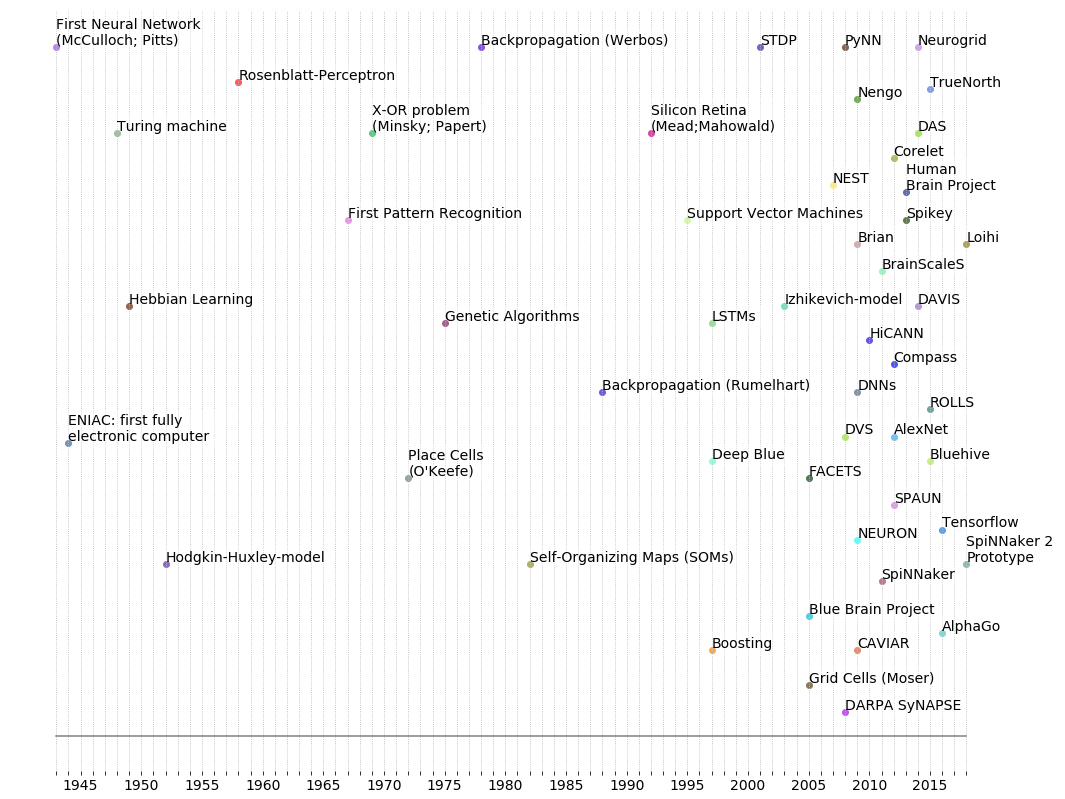
\includegraphics[width=0.95\textwidth,height=270px]{imgs/Neuromorphic_Timeline_beta.png}
	\caption{A selection of historical milestones in artificial intelligence, neuromorphic engineering and computational neuroscience. There is a significant boost of research and technologies in recent years.}
	\label{fig:neuro_time}
\end{figure*}
The research field of \aclp{ANN} goes back to the 1940s when McCulloch and Pitts introduced artificial neurons as computational units \cite{McCulloch1943}, which embody a simplified model of biological neurons.
These first simple networks were able to calculate compositions of basic logic functions \cite{McCulloch1943, Rojas1996}.
Rosenblatt \cite{Rosenblatt58} proposed the first neural network, which was capable of learning, by adding numerical weights to the connections of the network with threshold functions as activation functions: the \textit{perceptron}.
Minsky and Papert \cite{Minsky1969} showed, that single-layer perceptrons are not able to calculate an XOR-function or, more generally, are only capable of learning linearly separable patterns.
This caused a decreased interest in neural networks research until the rediscovery of the backpropagation algorithm \cite{Werbos1974} in the 1980s \cite{Rumelhart1986}, which introduced a practically feasible method to optimize the network weights using gradient descent and led to a resurgence of neural network research.
%This gradient descent called for continuous activation functions (mostly sigmoid or hyperbolic) instead of threshold-functions as activation functions, which made the so-called second generation \ac{ANN} universal approximators for continuous functions \cite{Cybenko1989}.
Since then, various different network architectures like feed-forward, \acp{CNN}, \acp{RNN}, \acp{RBF}, \acp{RBM}, \acp{SOM} and \ac{ART} just to name a few \cite{Schmidhuber2015} have been proposed for different learning paradigms.
Although several simpler methods like Boosting \cite{Freund1997} or \acp{SVM} \cite{Vapnik1995} have been developed and achieved noteworthy results, the availability of powerful, parallel computing hardware like \acp{GPU} as well as the advent and success  of deep learning (partly achieving better-than-human accuracy) made \acp{ANN} \cite{Rojas1996} and especially \acp{DNN} \cite{LeCun2015} the state-of-the-art for several machine learning tasks like visual digit \cite{Ciresan2012a} and traffic sign \cite{Ciresan2012} recognition in recent years.
Another great achievement in the field of deep learning was the victory of AlphaGo \cite{Silver2016} over the world's best Go player Lee Sedol in March 2016, which was considered to be at least a decade away due to the complexity of Go.
Compared to Deep Blue, the system that beat former chess world champion Garri Kasparov in 1997 \cite{Hsu2002} with sheer computational power by brute forcing through a large number of possible moves in advance to find the best one, this strategy is not feasible for Go due to its higher complexity (larger board, more options to consider per move).
In contrast, modern \acp{DNN} trained by a combination of supervised learning from human expert games and reinforcement learning from self-play have been used for the evaluation of board positions and selection of moves to avoid expensive look-ahead search \cite{Silver2016}.
A comprehensive and historical overview of relevant literature concerning \acp{ANN} and especially \acp{DNN} can be found in \cite{Schmidhuber2015, LeCun2015}.

\subsubsection{Neuromorphic systems}

The term neuromorphic itself was first introduced by Carver Mead in the late 1980s \cite{Mead90}, when describing one of the first silicon retinas.
He called artificial systems that share organization principles with biological nervous systems neuromorphic.
An interesting prototype of a silicon retina, which is now considered a milestone, was implemented by Misha Mahowald, a PhD student of Carver Mead.
Her thesis received Caltech's Milton and Francis Clauser Doctoral Prize for its originality and potential for opening up new avenues of human thought and endeavor.

Since these early days of neuromorphic engineering, the term has widely been used to describe \ac{VLSI} systems \cite{Mead1989}, novel computing devices \cite{Schemmel2010}, sensory systems \cite{Lichtsteiner2008, Liu2010}, software \cite{Davison2008, Bekolay2014} and algorithms \cite{ReverterValeiras2016}.
Considering the number of scientists, neuromorphic engineering is still a comparably young field of research but received an increased interest during the last decade from both academic and industrial research groups caused by the funding of large, ambitious projects.
Although there have been several achievements in the field during the 1990s \cite{Mead1989, Mahowald1992, Indiveri1997, Cauwenberghs1998} and early 2000s \cite{Liu2002}, the \ac{FACETS} project \cite{FACETS-proj} and the \ac{BBP} \cite{BlueBrain-proj}, both starting in 2005 and mainly funded by the \ac{EU} under the FP6-\ac{FET} program, were among the first big-budget neuromorphic projects.
The follow-up project \ac{BrainScaleS} \cite{BrainScaleS-proj, Schemmel2010} (2011-2015) built on and extended the research conducted during the \ac{FACETS} project.
The main developments of the \ac{FACETS} and \ac{BrainScaleS} projects are the \ac{HICANN} chip \cite{Schemmel2010} and the Python-based simulator-independent language \ac{PyNN} \cite{Davison2008} for building neural network models.
Building on \ac{BBP} the \ac{BrainScaleS} hardware development is currently continued in the neuromorphic computing platform of \ac{HBP} \cite{HBP-proj, Calimera2013}, a large ten-year research project, which was selected as one of the two \ac{EU}-\ac{FET} flagships in 2013 and is granted around one billion euros funding.
Another project starting in 2005, initially funded by the UK government until 2014 and now also part of the neuromorphic computing platform of \ac{HBP}, is the \ac{SpiNNaker} project \cite{Furber2014} during which the neuromorphic computing hardware of the same name was developed.
The \ac{HBP} is organized in thirteen platforms in total, which focus on different research fields related to the brain like for example theoretical neuroscience, neurorobotics, cognitive architectures, high performance computing, brain simulation and the aforementioned neuromorphic computing platform (see \cite{HBP-proj} for details).

Beside these research activities in Europe, the \ac{DARPA} funded another big-budget neuromorphic project: the \ac{SyNAPSE} program \cite{SYNAPSE-proj, Srinivasa2012}, which started in 2008 and is scheduled to run until 2016, has received 102.6 million US dollars in funding as of January 2013.
The program aims to build an electronic microprocessor system that matches a mammalian brain in function, size, and power consumption.
Achievements during the \ac{SyNAPSE} program, which is primarily contracted to IBM Research and \acs{HRL}, so far are include brain simulations, design of brain-inspired neuromorphic architectures \cite{Nere2012} and the development of a digital neuro-synaptic core \cite{Merolla2011}, which is a building block of IBM's recently published TrueNorth chip \cite{Akopyan2015}.
Further project results are the Corelet language \cite{Amir2013} and the simulator Compass \cite{Preissl2012}, which enable dedicated software development as well as simulation and testing of TrueNorth algorithms on standard hardware respectively.

Beside these projects, the neuromorphic community is coming together at two annual  workshops in Telluride and CapoCaccia, which have been established in 1994 and 2007 respectively, to discuss the current state of research in lectures and interactive talk sessions, to forge new ideas and to work on hands-on projects in small work groups.

%----------------------------------------------------------------------------------------------------------
\subsection{\aclp{SNN}}
\label{subsec:SNN}
%----------------------------------------------------------------------------------------------------------
\begin{figure}[t!]
	\centering
	\resizebox{.9\textwidth}{!}{%
		\subfloat[\label{subfig:biological_neuron}]{%
			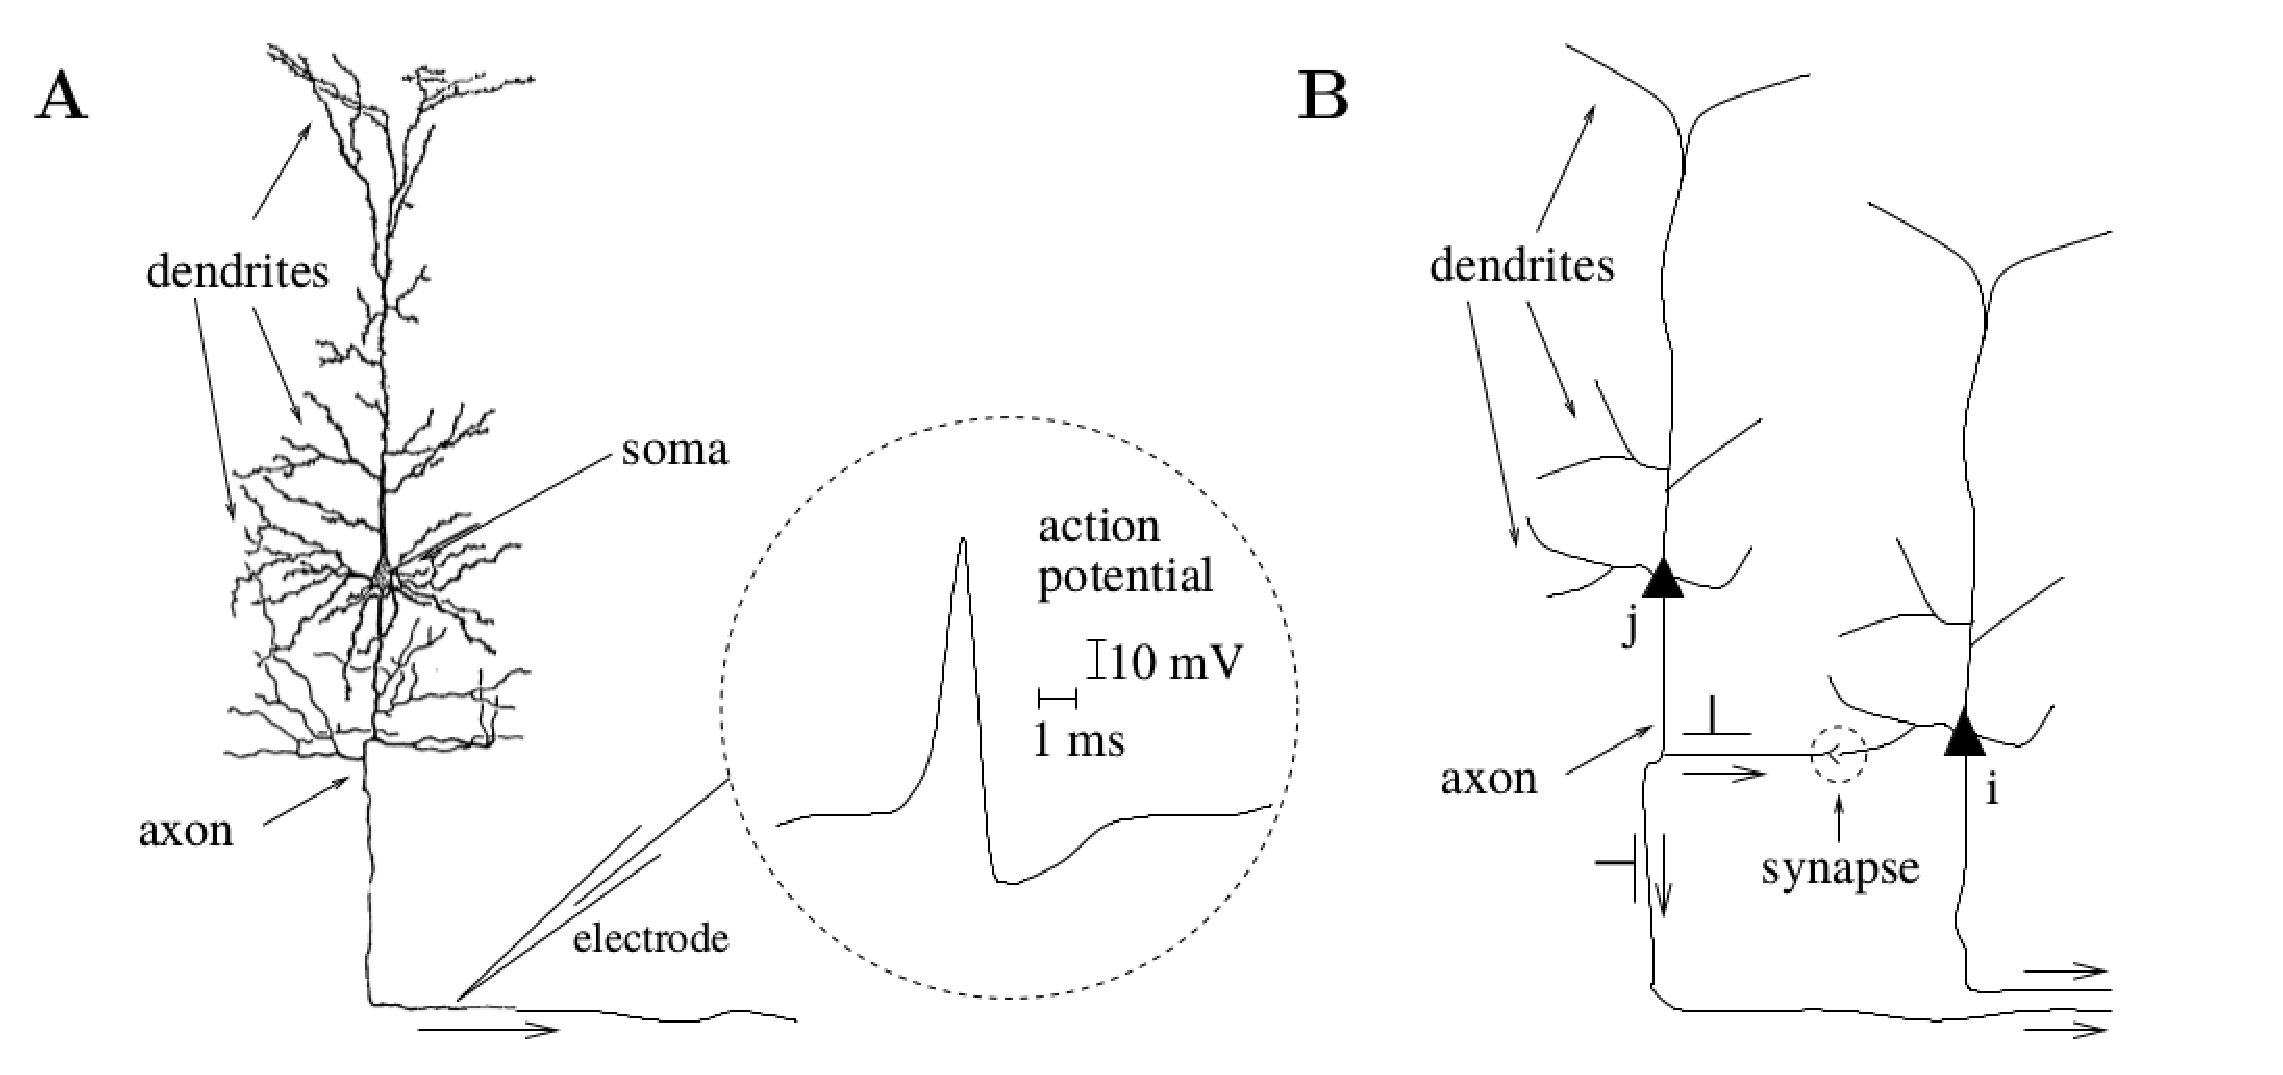
\includegraphics[height=3cm]{imgs/Neuron_model.eps}
		}
		\subfloat[\label{subfig:lif_neuron_model}]{%
			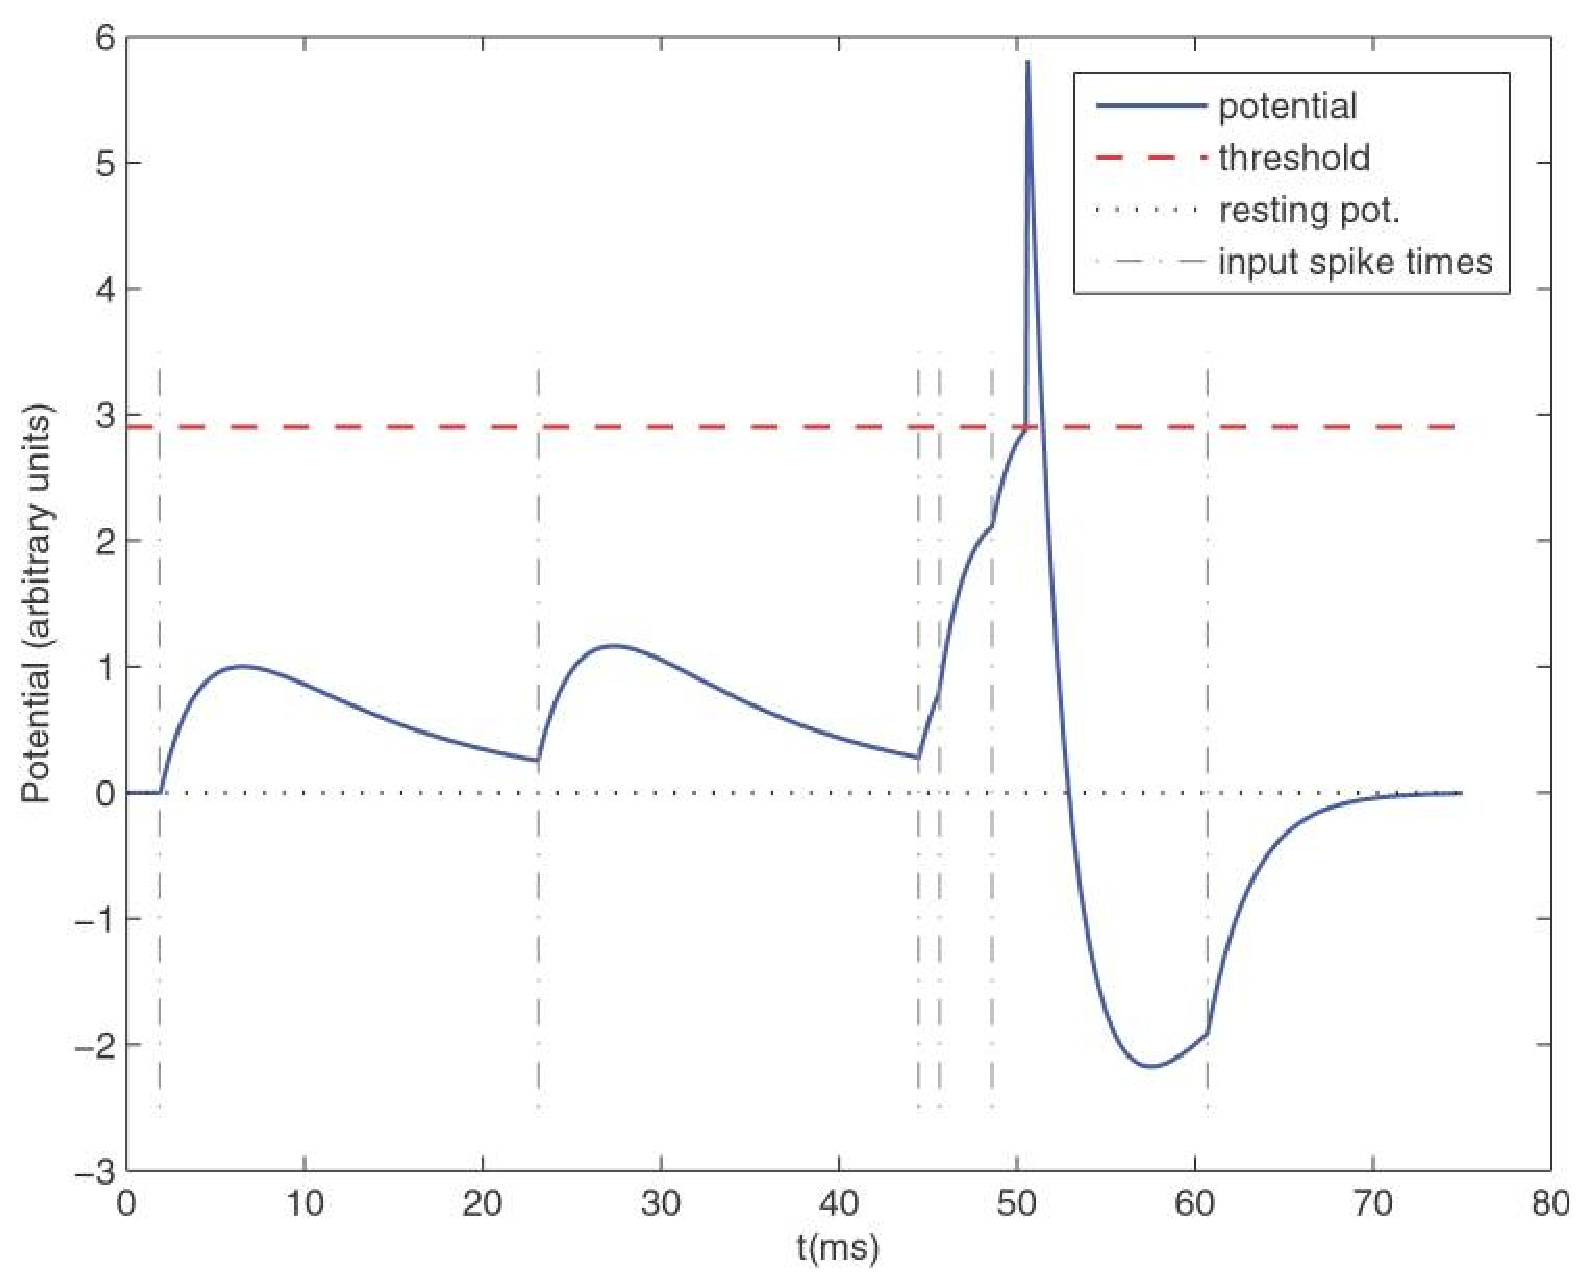
\includegraphics[height=3cm]{imgs/LIF_Neuron.eps}
		}
	}
    \caption{Visualization of different aspects of neuron models.~\protect\subref{subfig:biological_neuron} depicts the structure and functioning of biological neurons in a schematic visualization (image source \cite{Gerstner2002}).~\protect\subref{subfig:lif_neuron_model} visualizes the membrane potential's sub-threshold behavior of a \ac{LIF} neuron model (image source \cite{Masquelier2007}).}\label{fig:neuron_models}
\end{figure}

Fig.~\ref{subfig:biological_neuron} depicts the structure and functioning principles of biological neurons.
They  exchange information by sending short and sudden pulses, so-called action potentials or spikes via synaptic connections.
Whenever the membrane potential of a neuron, which can be increased or decreased by incoming spikes depending on the synaptic weight, reaches a certain threshold, the neuron produces a spike itself and resets its membrane potential afterwards \cite{Gerstner2002, Paugam2009}.
Recent neuroscientific research suggests that the exact timing of those spikes encodes information rather than just average firing rates \cite{Bohte2004}.
While traditional \acp{ANN} used in machine learning neglect these biological details, \acp{SNN} embody these spike times and are therefore often referred to as the third generation of neural networks \cite{Maass1997, Paugam2009}.
Maass showed in \cite{Maass1997}, that \acp{SNN} have at least the same computational power as threshold and sigmoidal neural networks of similar size.

The simplest spiking neuron model is the \acf{LIF} model with
\begin{equation}
\frac{\partial V}{\partial t}(t) = - \frac{1}{\tau_{m}} \left( V\left(t\right) - R \cdot I\left(t\right) \right)
\label{eq:LIF}
\end{equation}
describing the sub-threshold behavior of the neuron, where $V$ is the voltage across the membrane, $I(t)$ is the input current, $R$ is the passive membrane resistance and $\tau_{m}$ is the membrane time constant.
In other words, equation \ref{eq:LIF} states as follows: the membrane voltage increases in the presence of input current $I(t)$ depending on the membrane resistance $R$ while at the same time, especially in the absence of input current ($I(t)=0$), the voltage decreases or "leaks out" depending on the membrane time constant $\tau_{m}$.
When the voltage $V(t)$ passes a certain threshold $\vartheta$, the neuron produces a spike and the voltage is reset to a resting state $c$ for a certain refractory time interval $\tau_{ref}$ during which incoming spikes have no impact on the membrane potential.
Figure \ref{subfig:lif_neuron_model} visualizes the spiking behavior of the \ac{LIF} model.
It shows an example curve of the membrane potential of one \ac{LIF} neuron based on six incoming spikes whereas only the third, fourth and fifth incoming spike are appearing closely enough for the membrane potential to surpass it threshold and, therefore, cause the neuron to emit a spike itself.
The \ac{LIF} model, despite its biological simplifications, is maybe the most widely used neuron model for simulations due to its simplicity and comparably low computational complexity \cite{Izhikevich2004}, which allows simulations of large networks of neurons in reasonable time.
In contrast, the famous Hodgin-Huxley-model \cite{Hodgkin1952} with its four differential equations and dozens of (biologically meaningful) parameters is the model of high biological plausibility but also computationally challenging regarding large simulations \cite{Izhikevich2004}.
In 2003, Izhikevich proposed a neuron model \cite{Izhikevich2003} as compromise between biological plausibility and computational feasibility.
He showed that this simple model, described by two differential equations with four parameters, is able to produce all known spiking behaviors observed in cortical neurons \cite{Izhikevich2004}. 

One major hindrance for the widespread adoption of \acp{SNN} has been the problem, that standard learning algorithms for traditional \acp{ANN} like backpropagation \cite{Werbos1974} can not be directly applied to \acp{SNN}.
Although an analogon, the so-called SpikeProp algorithm \cite{Bohte2002} for \acp{SNN} has been developed, the more natural approach is to transfer and mimic biologically inspired learning approaches like Hebbian learning \cite{Hebb1949} or \ac{STDP} \cite{Bi2001}.
An overview of several learning approaches for \acp{SNN} possibly applied with neuromorphic hardware can be found in \cite{Walter2015}.
Another possibility is to train a traditional \ac{ANN} and convert the resulting network into a \ac{SNN} \cite{Diehl2015, Hunsberger2015}.
An example for this approach is the network performing the visual digit recognition task as part of the larger \ac{Spaun} model \cite{Eliasmith2012}, which was derived by training a \ac{DNN} consisting of four \ac{RBM} layers and converting this network using the principles of the \ac{NEF} \cite{Eliasmith2003}.
Although theoretically superior \cite{Maass1997}, \acp{SNN} have not yet outperformed state-of-the-art \acp{DNN} in terms of accuracy in practical machine learning applications \cite{Schmidhuber2015}.

Beside the aforementioned procedures to solve traditional machine learning tasks with \acp{SNN} and thereby encode artificial functions in spiking neurons, a different approach is to try to understand how complex cognitive behaviors and the underlying neural functions are performed in the brain.
Therefore, the question how the brain encodes complex information and behavior in trains of spikes and also how to decode these spike trains to reconstruct the encoded information needs to be answered.
Although modern research has shed some light on this question regarding the neural code, it is still mainly unanswered as we do not fully understand the anatomical and neurophysiological processes within the brain \cite{Stanley2013}.
Currently, there exist several approaches to code information as spike trains, which can be summarized by the categories rate coding, temporal coding \cite[Chap. 7.6]{Gerstner2014}, population coding \cite[Chap. 1]{Gerstner2002}, \cite{Ponulak2011, Boerlin2011} or sparse coding \cite{Olshausen1996}.
Except for the biologically unrealistic rate coding approach, there are cues for all of these coding schemes and even combinations \cite{Gupta2014} of them to appear in biological systems.

\subsubsection{Software tools}

There exist several different programming languages, simulators and software libraries specifically designed for modeling \acp{SNN} varying from tools like Corelet \cite{Amir2013} and Compass \cite{Preissl2012} working with one specific hardware component, in this case IBM's TrueNorth chip \cite{Akopyan2015} (cf. Sec. \ref{sec:neuromorphic_HW}), to libraries like \ac{PyNN} \cite{Davison2008}, which aim for universality to work with different simulators and hardware components as back-end.

The simulation tool offering maybe the highest level of abstraction is \ac{Nengo} \cite{Stewart2009}, which implements the principles of the \ac{NEF} \cite{Eliasmith2003} and was used to build the \ac{Spaun} model \cite{Eliasmith2012}.
Originally written in Java, \ac{Nengo} was re-implemented in Python \cite{Bekolay2014} and improved by incorporating the lessons learned from the creation of \ac{Spaun}.
\ac{Nengo} allows the user to describe a model on a high level of abstraction by defining groups of neurons to simulate different functional blocks while \ac{Nengo} takes care of neural properties and synaptic weights using the \ac{NEF} (see Sec. \ref{sec:neural_eng} for more details).
\ac{Nengo} models can be run using the internal simulation back-end, but also simulation on some neuromorphic hardware components like Neurogrid \cite{Dethier2011, Choudhary2012} and \ac{SpiNNaker} \cite{Mundy2015}, which are currently used in developments aiming to run the \ac{Spaun} model in real-time, is supported.

Another Python-based tool is \ac{PyNN} \cite{Davies2010}, which was developed during the \ac{FACETS} \cite{FACETS-proj} and \ac{BrainScaleS} \cite{BrainScaleS-proj} projects and aims for building \ac{SNN} models independent of actual simulation tools.
The level of abstraction is lower than \ac{Nengo}, but therefore it allows the creation of arbitrary neuron populations and connections, while the properties and synaptic weights need to be specified by the user or acquired using a learning algorithm.
\ac{PyNN} implements a number of standard models of neurons like \ac{LIF} or Izhikevich, connection algorithms like "one to one", "all to all" or connection matrices, static and plastic synapse types as well as several \ac{STDP} rules supported by the simulation and hardware back-ends.
Furthermore, \ac{PyNN} enables the user to implement custom models, connections and learning rules for advanced simulations and thereby extend the neural modeling toolkit.
\ac{PyNN} currently supports several different back-ends, e.g., simulators such as \ac{NEST} \cite{Gewaltig2007}, Brian \cite{Goodman2009} and NEURON  \cite{Carnevale2009} as well as neuromorphic hardware.
\ac{PyNN} is currently the preferred development environment for the creation of \ac{SNN} models to run on the \ac{SpiNNaker} system \cite{Furber2014}.
The mapping of the network structure, neurons and synapses to actual cores on the chip is done with a separate software package called \ac{PACMAN} \cite{Galluppi2012}.

Another Python-based software package which, in contrast to \ac{PyNN} and \ac{Nengo}, mainly aims at modularity and flexibility in terms of supporting as many different neuromorphic hardware systems as possible as a front-end is \ac{PyNCS} \cite{Stefanini2014}.

A comprehensive overview of several other simulation tools for neural modeling can be found in \cite{Brette2007}.

%----------------------------------------------------------------------------------------------------------
\subsection{Neuromorphic Hardware}
\label{sec:neuromorphic_HW}
%----------------------------------------------------------------------------------------------------------

In this section, we give a brief overview of recent neuromorphic prototypes and hardware developments.
Although we do not integrate the models and approaches developed in this thesis with this kind of dedicated hardware platforms, deployment on specialized hardware components is an interesting future possibility promising increased energy-efficiency and scalability.
The neuromorphic prototypes described here are still comparatively young and not technologically mature yet, especially compared to traditional computing systems.
Therefore, most of the hardware and sensors described are mainly developed and used in academic research and are not standardized, commercial products yet.
However, this technology is gradually becoming available to a broader community and draws increased attention in industrial research groups.

\subsubsection{Digital Neurochips}

\acp{GPU} provide a \ac{SIMD} architecture, which processes data in parallel at the cost of increased power consumption \cite{Krichmar2011, Carlson2014} compared to \acp{CPU}.
Allowing fast matrix and vector multiplication, \acp{GPU} provide an appealing platform for training and executing deep learning techniques \cite{Schmidhuber2015} on real-time data.
For specific applications, which take several months of training on a traditional \acp{CPU}, \ac{GPU}-based systems can significantly accelerate processing by several orders of magnitude to decrease the computation time to a number of days \cite{Edwards2015}.
A collaboration between NVIDIA and Stanford researchers demonstrated a cluster of \ac{GPU} servers, which was able to train a network with billion parameters (scalable to \num{11} billion using \num{16} machines) on just three computers in two days.
Each machine contained \num{4} NVIDIA GTX680 \acp{GPU} with \SI{4}{\giga\byte} at \SI{1}{\tera\nothing}\ac{FLOPS} each.

One of the recent developments in digital neuro-chips is IBM's TrueNorth \cite{Akopyan2015}.
It contains a network of \num{4096} cores with \num{256} digital neurons each following a digital, re-configurable spiking neuron model \cite{Cassidy2013} yielding the capability to implement over one million neurons and \num{256} million synapses in total while consuming only \SI{65}{\milli\watt} of power.
The cores are connected internally by a two-dimensional grid.
The intersections of this grid contain routers, which control the signal transmission within the network of cores inside a chip.
For programming this novel hardware implementation, a specialized programming language named Corelet was developed \cite{Amir2013}.

Another example of a digital neuromorphic hardware implementation is University of Manchester's \ac{SpiNNaker} system \cite{Furber2014}.
It contains \num{18} synchronously connected ARM968 microprocessors and \SI{128}{\mega\byte} \ac{DDR} \ac{SDRAM}.
Communication is carried out by a packet-switched on-chip network with all chips having their own router.
This architecture scales well to larger application by allowing to place more chips on a board \cite{Painkras2013,Navaridas2009}.
A \ac{SpiNNaker} system forms a toroidal mesh, which, despite having fixed connections, allows the simulation of neural networks of arbitrary connectivity due to the protocol implemented by the routers on the individual chips.

Another recent digital neuromorphic hardware platform is Intel's Loihi chip \cite{Davies2018}.
This chip consists of a fully asynchronous many-core mesh of \num{128} neuromorphic cores, each containing \num{1024} primitive units implementing spiking neuron behavior in a tree-like structure.
In total, it contains \num{130000} artificial spiking neurons and \num{130} million synapses.
One of Loihi's key features is the ability of on-chip learning, which is realized through a learning engine integrated in each core that enables the implementation of learning rules to adapt parameters of the core's \ac{SNN}.

\subsubsection{Analog Neurochips}

Most analog chips prohibit on-chip training due to limited adaptability of implementation techniques like capacitors \cite{Schwartz1990}, floating gate transistors \cite{Holler1989} or \acp{CCD} \cite{Agranat1990}.
On the other hand, analog techniques use less components and offer high-speed operation.
To exploit the benefits of analog semiconductor technologies and neural adaptivity, the learning algorithms have to be implemented on-chip.
However, on-chip-implementation limits the platform's re-configurability and complicates the implementation of most learning rules directly into analog \ac{VLSI} at the same time.
These limitations restrict the flexibility of analog designs compared to their digital counterparts.
%They possess similar functional properties as that of biological networks and can be interfaced directly with real analog world \cite{Mead90}.

The \ac{HICANN} chip \cite{Schemmel2008} has the capability to simulate \num{131072} synapses and \num{512} neurons residing inside an \ac{ANC}.
To simulate large networks, a wafer-scale integration method was used, which allows \num{384} \ac{HICANN} chips to be interconnected on a wafer of \SI{20}{\centi\meter} diameter \cite{Schemmel2010}.
The spikes between various \acp{ANC} on a wafer and between interconnected wafers are carried out by a network of horizontal and vertical grid like structure.
The horizontal pathway consists of \num{64} bus lines which carry spikes from \num{64} neurons.
The \num{256} vertical lines collect spikes for all connected \acp{ANC}.
The spikes are represented as data packet of \SI{6}{\bit} for groups of \num{64} neurons and transmitted using \ac{AER}. 

The \ac{ROLLS} neuromorphic processor consists of \num{256} neurons and \num{128000} synapses.
It consumes only \SI{4}{\milli\watt} of power and uses exponential \ac{IF} modeling \cite{Qiao2015}.
The latest processor contains different configuration options.
Each neural circuit is connected to three different types of synaptic circuits: the first is an array of $256\times256$ synapse, which can be excitatory or inhibitory.
The synapses in the second $256\times256$ array offers only excitatory mode.
In the third array, there are $256\times2$ virtual synapses with weights being configurable as both, excitatory as well as inhibitory.
The virtual synapses operate in shared mode and occupy less space compared to individual circuits.
The neural spikes are generated and transmitted using an \ac{AER} protocol with \SI{8}{\bit} neuron addresses \cite{Qiao2015}.

Another example of analog neural hardware is a chip \cite{Srinivasa2012} developed under \ac{DARPA}-funded \ac{HRL} \ac{SyNAPSE} project, which uses \ac{STM} for computation and memristors for synaptic weights storage.
It contains a total of \num{576} neurons and \num{73728} synapses, arranged in an array of $24\times24$ neurons each with \num{128} synapses and consumes \SI{130}{\milli\watt}.
In \ac{STM} methodology, a single synaptic circuit on the chip calculates multiple logical synapses of the simulated neural network since the electrical circuitry can function at higher speeds than biological neurons.
Hence, a single synaptic circuit allows emulating multiple logical synapses by switching between the corresponding parameter sets.
There is a point-to-point routing mechanism avoiding the necessity of the \ac{AER} protocol \cite{Walter2015}. 

The Brain in Silicon group at Stanford University developed the custom board Neurogrid, which contains \num{16} Neurocores \cite{Benjamin2014, Choudhary2012}.
The neuron circuits are arranged in a $256\times256$ grid with every neuron having separate circuits for its soma and  dendrite and combining analog computations with digital communication.
The system is capable of simulating a million neurons and eight billion synapses in real-time while consuming \SI{3.1}{\watt} of power.
Neurogrid employs the \ac{AER} protocol to transmit spikes.
It additionally implements a deadlock-free wormhole routing protocol to ensure free transmission of packets.
Finally, Neurogrid allows to explore different cortical areas of the brain by programming each of the Neurocores with a different model \cite{Merolla2014}.

\subsubsection{Neuromorphic Sensors}
\label{subsubsec:neuro_sensors}

\begin{figure}[t!]
	\centering
	\subfloat[]{\label{subfig:DVS_rotationg_dot}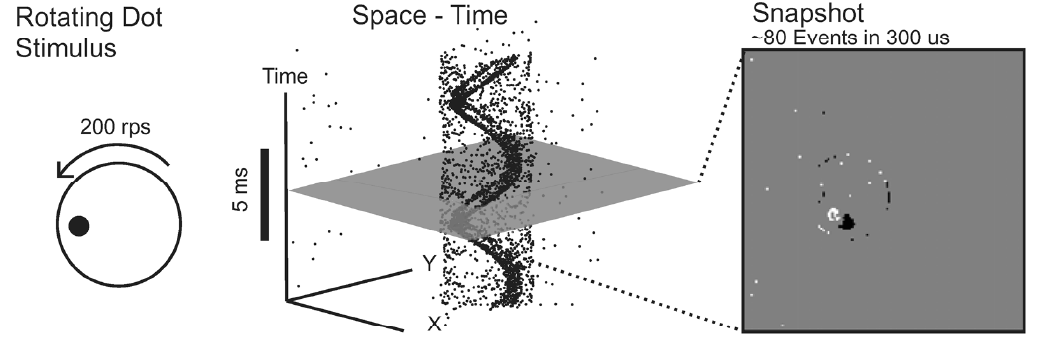
\includegraphics[width=0.9\textwidth]{imgs/DVS_rotating_dot_stimulus.PNG}}
	\par\medskip
	\begin{minipage}{.48\columnwidth}
		\centering
		\subfloat[]{\label{subfig:DVS_pixel_core}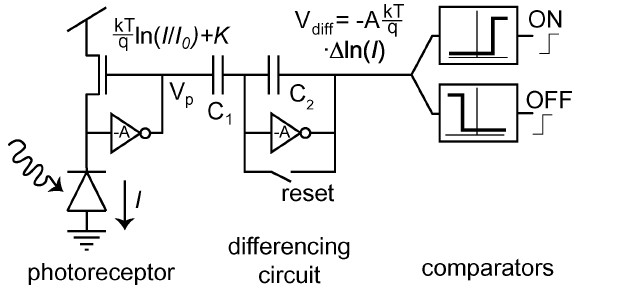
\includegraphics[width=1.15\textwidth]{imgs/DVS_pixel_core.PNG}}
	\end{minipage}%
	\begin{minipage}{.48\columnwidth}
		\centering
		\subfloat[]{\label{subfig:DVS_operation_principle}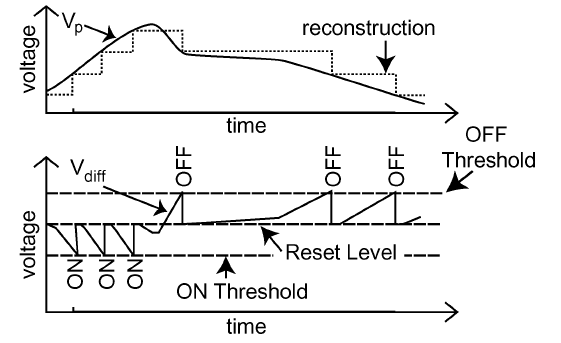
\includegraphics[width=0.9\textwidth]{imgs/DVS_operation_principle.PNG}}
	\end{minipage}\par\medskip
	\caption{(a) Space-time representation of the event stream generated by a rotating dot on a spinning disk and a snapshot of the events (b) abstracted pixel core schematic (c) principle operation of single \ac{DVS} pixel. Image source: \cite{Lichtsteiner2008}}
	\label{fig:DVS_with_schem}
\end{figure}
To integrate neuromorphic hardware in real-world applications such as neurorobotics, it needs to be able to process sensors signals.
The neurally inspired, non von-Neumannian architecture requires either a new generation of sensors such as the \ac{DVS} \cite{Lichtsteiner2008}, \ac{DAVIS} \cite{Brandli2014} or \ac{DAS} \cite{Liu2014}, which already embody the spiking neuron signal processing, or a way of translating traditional sensor signals to sequences of spikes.
Several approaches to encode signals and stimuli with trains of spikes, e.g., by rate coding, temporal coding \cite[Chap. 7.6]{Gerstner2014} or population coding \cite[Chap. 1]{Gerstner2002}, \cite{Ponulak2011} have been investigated.
Neuromorphic sensors on the other hand, directly emit a sequence of events without the need of such a translation process.
The \ac{DVS} for example, unlike traditional frame-based cameras, generates spike events \cite{Lichtsteiner2008} asynchronously for individual pixels when perceiving relative illumination changes (see Fig. \ref{fig:DVS_with_schem}), which are key features of biological vision \cite{Lichtsteiner2008}.
This event-based approach offers several advantages compared to conventional frame-based cameras like the ability to perceive very fast movements (sub-millisecond time precision) without the need to wait for the next frame and the time to process it
Furthermore, the rate of the output data depends on the dynamic content of the scene (Fig. \ref{subfig:DVS_rotationg_dot}) and thus reduces the output of redundant information at a fixed frame-rate.

The \ac{DVS}-pixels were designed to cover wide dynamic range and to offer low latency and mismatch.
This is achieved by a fast photoreceptor circuit with logarithmic response whose output is fed into a high precision difference amplifier circuit followed by a two-transistor comparator circuit (see Fig. \ref{subfig:DVS_pixel_core} and \ref{subfig:DVS_operation_principle}).
%The pixels are arranged in rows and columns which have $x$, $y$-address.
The comparator circuit produces ON and OFF signals for each pixel, which are passed to the \ac{AER} interface for transmission \cite{Lichtsteiner2008}.
On the other hand, the \ac{DAVIS} employs an \ac{APS} circuit to output synchronous global shutter frames, which helps in persevering absolute intensity information needed for classification and object recognition tasks while asynchronous \ac{DVS} events are beneficial for the tracking of fast moving objects \cite{Brandli2014}.

\subsection{Neuromorphic Applications}
\label{subsec:neuro_applic}

In this section we present some examples of applications of neuromorphic hardware and sensors described in Sec. \ref{sec:neuromorphic_HW}, software, algorithms and neural modeling depicted in Sec. \ref{subsec:SNN} as well as combinations of both.
First, we describe applications using either neuromorphic sensors or hardware in combination with traditional computing hardware.
Then, we focus on purely neuromorphic systems, where the spiking signals of neuromorphic sensors, mainly the \ac{DVS}, is processed by neuromorphic hardware.
Although there are currently - to the knowledge of the author - no neuromorphic actuators working directly on the basis of spikes, we refer to the robotic systems described here as purely neuromorphic.

\subsubsection{Mixed systems}
\label{subsubsec:mixed_sys}

Neuromorphic vision \cite{Tan2015} is an emerging field of research, which aims to transfer approaches from traditional computer vision and also establish new methods incorporating the characteristics of the \ac{DVS}.
To perform pattern recognition tasks with neuromorphic cameras and at the same time use traditional methods as a benchmark, existing image data bases like the \ac{MNIST} data set \cite{LeCun1998} are translated to neuromorphic data sets by presenting the images on a computer screen to a \ac{DVS} sensor moving minimally back and forth \cite{Orchard2015} (mimicking saccade movements of the human eye), which gives better results than moving the images themselves on the screen \cite{Serrano-Gotarredona2013}.

As the \ac{DVS} naturally captures moving objects when held statically and cues of the ego-motion when moving, tracking of these movements are suitable applications making use of the sensor's characteristics.
These characteristics along with the \ac{DVS}'s advantages compared to traditional frame-based cameras, which have been described in Sec. \ref{subsubsec:neuro_sensors}, have been demonstrated in applications like pencil balancing \cite{Conradt2009} and a robotic goalie \cite{Delbruck2013} interfacing the \ac{DVS} with traditional computing hardware and actuators.
Keeping track of (geometric) features \cite{Lagorce2015} and contours \cite{Barranco2014} observed by the \ac{DVS} lays the foundation for more sophisticated algorithms.
Researchers recently proposed several approaches for tracking people \cite{Schraml2010, Piatkowska2012} and other geometric objects \cite{ReverterValeiras2016} using stationary sensors.
Especially tracking at high velocities \cite{Saner2014} benefits largely from the sub-millisecond time precision of the \ac{DVS} even enabling tracking of particles in fluid flows \cite{Drazen2011}, which would require a high-speed PC, lots of disk space and high-intensity laser strobe lighting to illuminate the fluid in a conventional setting.

A traditional application of computer vision in robotics is the estimation of the ego-motion or odometry based on optical flow (an event-based approach on optical flow can be found in \cite{Benosman2014}), which can also be obtained by combining traditional cameras with the \ac{DVS} on a small wheeled robot \cite{Censi2014}.
Another suitable application for the \ac{DVS} is the estimation and tracking of the whole six degree-of-freedom pose of a flying robot, especially when performing high-speed maneuvers, where traditional cameras suffer from motion blur \cite{Mueggler2014}.
Another problem in robotics closely related to tracking is self-localization of the robot using a given map of the environment or building a map online and localizing within this map at the same time, which is known as the \ac{SLAM} problem \cite{Thrun2005}.
Localization performed within a given map using the \ac{DVS} on ground vehicles and by tracking markers from a flying robot is presented in \cite{Gallego2015} and \cite{Censi2013} respectively.
There are also several papers treating the \ac{SLAM} problem \cite{Weikersdorfer2012, Weikersdorfer2014} or the related problem of tracking the camera pose and simultaneously reconstructing the observed scene by mosaicing \cite{Kim2014} with neuromorphic vision sensors.

Most of the tracking algorithms mentioned here use variations of traditional Bayesian filters like (extended) Kalman- or particle-filters \cite{Thrun2005} for consecutive estimation of the quantity of interest.
However, due to the asynchronous information processing of the \ac{DVS} or neuromorphic systems in general these filters need some modifications to work with this event-based approach \cite{Weikersdorfer2013} like taking several past measurements into account (in contrast to the traditional Markov assumption) or updating only after a certain number of events have occurred to avoid computational overhead.

In \cite{Axenie2015}, the authors describe a biologically inspired system for sensor-fusion of several traditional sensors like wheel encoders, magnetometer and gyroscope for ego-motion estimation demonstrated in ground and flying robots.
Another example for sensor fusion is presented in \cite{OConnor2013}, where the biologically inspired \ac{DVS} and \ac{DAS} sensors are used to recognize hand-written digits from the \ac{MNIST} data set \cite{LeCun1998}.
To incorporate the neuromorphic audio sensor, each digit is assigned one tone frequency in the A harmonic minor scale, while the actual fusion is performed by a \ac{DBN} consisting of several, pre-trained (unsupervised) \ac{RBM} layers, which was traditionally trained and afterwards transferred to an event-based network.
Although the authors state that the actual implementation in \cite{OConnor2013} is just a proof-of-concept in software, their approach shows promise to translate fully trained \acp{DBN} to \acp{SNN}, deploy them on efficient neuromorphic chips and thereby making this technology available for mobile and/or real-time applications.

To demonstrate the functionality and applicability of their neuromorphic chip TrueNorth, IBM implemented several proof-of-concept applications ranging from virtual robots, game simulations \cite{Arthur2012}, digit recognition \cite{Arthur2012, Esser2013} to classical machine learning tasks like object detection \cite{Akopyan2015}.
In \cite{Arthur2012} the authors present four example applications of neural algorithms implemented on TrueNorth using the Corelet language: a virtual robot driver aiming to keep the simulated robot on a virtual road based on visual cues, a neural algorithm controlling an autonomous player performing the classical video game pong, a neural implementation recognizing hand-written digits of the \ac{MNIST} data-base using \acp{RBM} as well as a Hopfield network, which performs auto-association.
Seven example algorithms and applications for TrueNorth are presented in \cite{Esser2013}: speaker recognition using \acp{CNN} on the \ac{CUAVE} data set \cite{Patterson2002}, composer recognition distinguishing between classical composers Bach and Beethoven using liquid state machines, recognition of hand-written digits of the \ac{MNIST} data set using population coding and \acp{RBM}, a neural implementation of a \ac{HMM}, collision avoidance using motion extraction and looming detection, optical flow based on \acp{CNN} and eye detection using the \ac{DVS}.
Most of these algorithms are simplified proof-of-concept implementations showing the general applicability of TrueNorth but are not competitive with traditional machine learning algorithms yet (e.g. \SI{92.34}{\percent} \cite{Esser2013} vs. \SI{99.77}{\percent} \cite{Ciresan2012a} correct classifications on \ac{MNIST}).
In \cite{Schmitt2017}, the authors demonstrate training and deployment of \acp{DNN} on the \ac{MNIST}-data set using the \ac{BrainScaleS} hardware.
A more sophisticated application is the multi object detection and classification task described in \cite{Akopyan2015}, which detects moving and stationary people, bicyclists, cars, buses and trucks from a HD video stream in real-time recorded by a stationary camera using Haar-like features, saccades, K-means- and Grid-classifiers.

The use of the neuromorphic hardware Neurogrid \cite{Benjamin2014} as computational back-end for \ac{Nengo} and proof-of-concept solution for medical motor-prostheses, which shall be connected to biological neurons and thereby be controlled by the patient's brain, is described in \cite{Choudhary2012} and \cite{Dethier2011} respectively.
The \ac{SpiNNaker} system \cite{Furber2014} also supports the simulation of neural models created using \ac{PyNN} or \ac{Nengo} \cite{Mundy2015}.
Furthermore, several neural network architectures like \acp{CNN} \cite{Serrano-Gotarredona2015} and pre-trained \acp{DBN} \cite{Stromatias2015, Stromatias2015a} have also been implemented on the \ac{SpiNNaker} system.
To enable biologically inspired learning like \ac{STDP} \cite{Bi2001}, according rules adapting the synaptic weights depending on the timing of the spikes have efficiently been implemented on the \ac{SpiNNaker} \cite{Diehl2014} chip as well.

\subsubsection{Purely neuromorphic systems}
\label{subsubsec:neuro_systems}

\begin{figure}[t!]
	\centering
	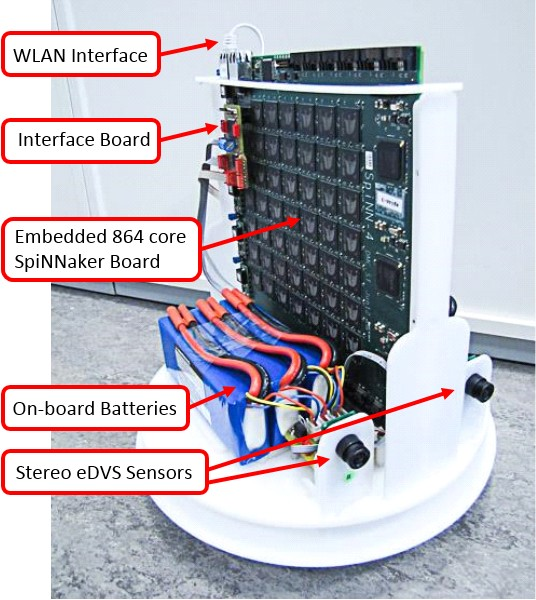
\includegraphics[width=0.48\textwidth]{imgs/SpinRobot.jpg}
	\caption{Example of a closed-loop, neuromorphic robotic system with two event-based embedded \acp{DVS} and a 48-node \ac{SpiNNaker} board. Image source: \cite{Galluppi2014}}
	\label{fig:spin_robot}
\end{figure}
Some examples of closed-loop systems deployed in small robots are presented in \cite{Davies2010, Denk2013, Galluppi2014}.
In \cite{Davies2010, Denk2013}, the authors interface two embedded \ac{DVS} cameras directly with a \ac{SpiNNaker} platform mounted on a small robot (see Fig. \ref{fig:spin_robot}).
The implemented neural networks enable simple autonomous behaviors like following a line \cite{Davies2010} or approaching a light stimulus \cite{Denk2013}.
In \cite{Galluppi2014}, a small robot with a similar setup is able to perform trajectory stabilization using optical flow from the \ac{DVS} cameras as input.
Another simple task described in \cite{Galluppi2014} is the recognition and tracking of a light stimulus and keeping the robot at a certain distance and angular orientation with regard to this stimulus.
The whole processing chain from visual perception over internal processing to motor control in these robot experiments are realized using spiking neuron models.
The neural implementation of the latter two applications are done in \ac{PyNN} and \ac{Nengo} respectively.

While the aforementioned sensorimotor behaviors are manually engineered, there are attempts to learn more sophisticated, complex behaviors from simpler basic movements \cite{Conradt2014, Stewart2016}.
These basic maneuvers are still manually engineered relating sensor cues to simple movements like driving forward with no obstacle in the sensors field of view, turning with an obstacle in in front of the robot or driving backwards when being close to an obstacle.
In \cite{Conradt2014} the authors describe a method on learning more sophisticated behaviors from recorded sensorimotor data obtained from driving the robot by remote control as training examples, which can be considered as a supervised learning approach.
In \cite{Stewart2016}, the training examples are taken from recording data of the robot driving around without human interference and just labeling those situations as positive examples when the robot performed the desired action by accident, which is considered as reinforcement learning.
Both approaches are implemented on a small robot with the \ac{DVS} as sensory input using \ac{Nengo} and the \ac{NEF} as well as its interface \cite{Mundy2015} for running neural networks models on the \ac{SpiNNaker} hardware \cite{Furber2014}.
% %----------------------------------------------------------------------------------------------------------
% \section{\aclp{ANN}}
% \label{sec:ML_ANN}
% %----------------------------------------------------------------------------------------------------------
% Machine learning in general is the science of constructing computer programs, which improve with experience.
% This is attractive if manually programming a desired functionality is not cost-efficient, intractable or simply impossible.
% The overall goal of machine learning algorithms is to generalize beyond examples, i.e. to generate models that describe the presented input sufficiently well to make the best possible prediction when confronted with previously unseen data.
% A formal, widely cited definition of machine learning has been presented by Thomas M. Mitchell in \cite{Mitchell1997}:
% \begin{defn}
% 	A computer program is said to \textbf{learn} from experience $E$ with respect to some class of tasks $T$ and performance measure $P$ if its performance at tasks in $T$, as measured by $P$, improves with experience $E$.
% \end{defn}
% A large body of research has focused on machine learning during the last decades.
% One major branch of machine learning are \acp{ANN} and \acp{DNN} in particular, which are currently the state-of-the-art of many machine learning tasks.
% \subsection{A brief history}
% \subsection{Supervised Learning}
% \todo[inline]{brief introduction to \acp{DNN} in general, particularly \acp{CNN} for classification, mentioning automotive related applications. Also mention \acp{RNN} and especially \ac{LSTM} as for time-series analysis/prediction as it is related to our behaviour prediction task}
% \subsection{Unsupervised Learning}
% \todo[inline]{brief introduction some unsupervised learning strategies. Focus especially on approaches to learn word embeddings like word2vec \cite{Mikolov2013}, GloVe \cite{Pennington2014}. Also mention problems of those approaches \cite{Levy2015}}
% \subsection{Reinforcement Learning}
% \todo[inline]{very brief introduction. Not sure yet if we need this secton at all}
%From the first theoretical considerations concerning artificial neural networks by McCulloc and Pitts(\todo{Citation}) in the 1940s and the first Multilayer-Perceptrons by Rosenblatt (\todo{Citation}) about a decade later, machine learning algorithms started to receive widespread attention with the rediscovery \cite{Rumelhart1988} of the well-known backpropagation algorithm \cite{Werbos1974}.
%Since then, several approaches to machine learning, apart from artificial neural networks, like AdaBoost (\todo{Citation}), Decision Trees (\todo{citation}), Bayesian Networks (\todo{citation}) or \ac{SVM} (\todo{citation Vapnik, V. (1995), The Nature of Statistical Learning Theory. Springer Verlag, Cristianini, N. and Shawe-Taylor, J. (2000). An Introduction to Support Vector Machines and Other Kernel-Based Learning Methods. Cambridge University Press, Cambridge}) have been proposed.
%These methods vary in representation of the data, the evaluation (or objective) function, the optimization technique and the learning paradigm.
%Through availability of larger datasets and increased computational power, machine learning has seen significant progress in recent years.
%The use of deep neural networks \cite{Schmidhuber2015}, enabled through modern, powerful computing hardware like \ac{GPU}, yielded a significant performance boost in several classification tasks.
%Today, modern deep learning algorithms can even rival human performance on different visual classification tasks like traffic sign \cite{Ciresan2012} or digit recognition \cite{Ciresan2012a}.
%
%So-called second generation \ac{ANN} introduced continuous (e.g. sigmoid or hyperbolic) instead of step- or threshold-functions (\todo{Citation}) as activation functions, which made them universal approximators for continuous functions \cite{Cybenko1989}.
%The term "neuromorphic" was first introduced by Carver Mead in \cite{Mead90}, when describing one of the first silicon retinas.
%For clarity, a first broad definition is provided, which will need some refinement while proceeding in this section:
%\begin{defn}
%\label{def:neuromorph}
%Artificial systems, that share organization principles with biological nervous systems are called \textbf{neuromorphic}.
%\end{defn}
%Biologically inspired systems and algorithms have seen significant progress and achieved remarkable results, e.g. in the field of machine learning, despite some simplifications in terms of biological accuracy.
%So-called first and second generation \ac{ANN} described in \ref{subsec:ML_ANN} are also covered by definition \ref{def:neuromorph} as neuromorphic systems, although they neglect some biological details.
%\subsection{Spiking Neural Networks}
%Biological neurons exchange information by sending short and sudden increases in their membrane voltage, so-called action potentials or spikes.
%Recent neurological research suggests that the exact timing of those spikes encodes information rather than just average firing rates (\todo{Citation}).
%While \ac{ANN} of the first two generations neglect these biological details, recent neural networks structures, so-called \ac{SNN} \cite{Paugam2009}, embody these spike times and are therefor often referred to as the third generation of neural networks .

\section{Cognitive Modeling}%
\label{sec:cognitive_modeling}

Over the last decades, understanding and building cognitive systems has seen extensive research leading to the development of several cognitive architectures.
A cognitive architecture is a "general proposal about the representation and processes that produce intelligent thought" \cite{Thagard2012}.
On the one hand, these architectures are used to explain and better understand important aspects of human behavior and intelligence.
However, they are also used to design computers and robots mimicking certain cognitive abilities of humans.
In this respect, cognitive architectures are typically clustered in three main categories, namely symbolism, connectionism and dynamicism \cite{Eliasmith2013}.
We will give a brief overview over symbolic and connectionist approaches in subsequent sections, whereas dynamicism \cite{Schoener2008} is of lower relevance to the work at hand.

One important aspect of cognitive modeling and, more generally, \ac{AI}, is knowledge representation.
Any intelligent agent, artificial or biological, that wants to perform reasoning about the world it encounters, needs to be able to build an internal representation of its perceived information.
This aspect is quite important for subsequent chapters, while a formal definition of what knowledge representation actually is appears to be difficult and thus is often avoided in the literature \cite{Davis1993}.
In \cite{Davis1993}, the authors describe five defining roles, that such a representation can play.
A representation is a surrogate, i.e., an internal substitute for a real-world entity and as such an imperfect approximation.
Therefore, the choice for each representation implies a set of ontological commitments, which effect the focus of attention of the representation.  
When the focus of such a representation is to enable some kind of reasoning in intelligent machines or robotic systems, these systems need to be able to manipulate the representation and perform computations with it.
Finally, as long as the machine needs to interact or communicate with humans in the sense that humans inform the machine about the world by e.g.\ creating a representation, this representation itself also plays the role of a medium of human expression.
Therefore, we put emphasis on the different aspects of knowledge representation in the different cognitive modeling architectures presented in this section.

\subsection{Symbolic approaches}%
\label{subsec:symbolic_approaches}

Symbolic approaches are often referred to as the "classical approach" to cognitive modeling or \acf{GOFAI}.
Most of the approaches rely on the metaphor of the "mind as computer", supposing that cognitive systems have a symbolic "language of thought" \cite{Fodor1975}, that expresses the rationale and rules the systems follow.
The corresponding analogue for computers are programming languages.
The dominant paradigm of such approaches is "the manipulation of discrete atomic symbols by explicit rules" \cite{Levy2008}.
The most prominent approaches in this category are production systems, which typically rely on if-then-rules (or productions) and a control structure.
One of the first and most influential achievements in this field is a program called the \ac{CogGPS}, which was able to to solve elementary problems in symbolic logic on its own.
The steps \ac{CogGPS} performed to solve a given problem often matched the steps reported by people solving the same problem.
This success enabled the development of several other cognitive architectures such as Soar \cite{Laird1987}, \ac{EPIC} \cite{Kieras1997} and \ac{ACT} \cite{Anderson1983} and its successor \ac{ACT-R} \cite{Anderson1996}, which all employed production systems at their core but adding their own extensions.
\ac{ACT-R} is the most modern of these architectures and arguably the most successful and thus most widely used cognitive architecture.
Although \ac{ACT-R} incorporates some connectionist-like mechanism in its memory system, it is widely considered a symbolic architectures as it relies on symbolic representations and a production system as central procedural core.
In general, symbolic approaches to cognitive modeling had the most success when addressing higher-level cognitive tasks, with a rigid set of rules and potential for pre-specified solutions.
However, these approaches are rarely used when it comes to real-time critic systems such as robots or if the system needs to generalize beyond pre-specified situations.

\subsection{Connectionist approaches}%
\label{subsec:connectionist_approaches}

One of the first theories challenging the paradigm of \ac{GOFAI} was the "Society of Mind" \cite{Minsky1986} view of specialized individual agents cooperating to accomplish a certain goal.
The strongest challenge however, was the emergence of connectionism \cite{Rumelhart1986a} (popularly referred to as neural networks), which offered novel learning algorithms such as backpropagation \cite{Rumelhart1986} to solve a wide variety of problems.
Connectionism explains cognitive phenomena by constructing models consisting of large networks of interconnected nodes performing rather simple input/output mappings.
If these nodes, however, are connected to sufficiently large networks, the nodes' activity is able to implement cognitive behavior such as rules or analyzing patterns.
We already gave a brief historical overview over the research conducted related to \acp{ANN} in section~\ref{subsec:history_neural_nets}. 
The metaphor behind connectionist approaches to cognitive modeling is that of the "mind as brain", as the processing employed in connectionism is often referred to as "brain-like" or "brain-inspired".
Connectionism has shown remarkable results in diverse applications such as computer vision, pattern recognition, sequential data analysis and language processing just to name a few.
However, the most serious criticism of connectionist approaches are that they could not exploit systematic, compositional representations or logical reasoning of the form used in \ac{GOFAI}. 
Furthermore, the nodes in connectionist networks typically simplify the computational and representational properties of biological neurons, which in addition to the biological implausibility of the backpropagation algorithm, concerns cognitive modelers interested in biological realism.
Finally, the ability to learn and derive internal representations of features from data, despite being one of the greatest strengths of neural networks approaches, is sometimes criticized for lack of comprehensibility.

\subsection{Vector-based approaches}%
\label{subsec:vector_based_approaches}

To address some of the concerns regarding both, symbolic and connectionist approaches to cognitive modeling, researchers developed a hybrid approach often referred to as \acf{VSA}, a class of connectionist distributed representations.
In chapter~\ref{chap:introduction_to_vsas}, we give an in-depth introduction to the theory and mathematical properties of \acp{VSA}, which will be import ingredients for the remainder of the thesis.
Here, we give a brief overview of the different variants of such architectures, their similarities and differences, related work and some applications.
All of the modeling approaches presented in this section employ (high-dimensional) vectors as representational units.
Similar to the representations derived from connectionist approaches, these are distributed representations, which offer nice properties such as robustness to noise and the support of distance metrics.
Additionally, all of the approaches allow to treat such vectors as "symbol-like" entities, which can be manipulated through the architecture's algebraic operations (see chapter~\ref{chap:introduction_to_vsas} for details).
The first attempt on structured vector representations used the tensor product as multiplication operation \cite{Smolensky1990} to bind two different vector together.
The tensor product approach already allows for an sufficiently complex embedded structure to do linguistic processing.
However, scaling becomes a problematic issues as each uncompressed tensor product operation of two high-dimensional vectors increases the result's dimension, which quickly becomes impracticable.
Hence, there are several architectures such as \ac{MAP} \cite{Gayler1998, Gayler2003}, \acp{BSC} \cite{Kanerva1988} and \acp{HRR} \cite{Plate1991, Plate1994}, which propose different compressed multiplication operations replacing the tensor product and resulting in vectors with the same dimension as the input vectors.
Furthermore, these different \ac{VSA} variants differ in the choice of the numerical space to pick the vectors' elements from, i.e., if they use binary, real- or complex-valued vectors. 
The \ac{SPA} \cite{Eliasmith2013} is built upon \acp{HRR} and extends these architectures, by proposing an efficient mechanism of implementing structured vector representations in populations of spiking neurons using the principles of the \ac{NEF} \cite{Eliasmith2003} (again, we refer to chapter~\ref{chap:introduction_to_vsas} and especially sections~\ref{sec:neural_eng} and~\ref{subsec:implementation_in_snns} for further details).   
This architecture has been used to built the currently largest functional model of a brain \cite{Eliasmith2012} using a combination of structured vector representations for symbol-like processing and a spiking neuron substrate.

The most prominent application of vector representations despite cognitive modeling \cite{Blouw2016, Crawford2016, Eliasmith2012} is language processing \cite{Gayler2003}.
In this context, word embedding refers to the problem of finding (or automatically learning) desirably meaningful representations for words.
Modern word embedding algorithms such as word2vec \cite{Mikolov2013, Mikolov2013b} or \ac{GloVe} \cite{Pennington2014} employ high-dimensional vectors as representational structure to encode words and language by learning in unsupervised fashion from large corpora of text.
There are also attempts of using such representations in other domains to e.g., better explain and quantify how \acp{DNN} learn and derive concepts \cite{Fong2018} or for embedding low-level vehicle sensor data in an abstract representation \cite{Hallac2018}.

Another approach employing vector representations is the work of companies such as Numenta \cite{Numenta} and Cortical.io \cite{Cortialio}.
They employ binary vector representations similar to \acp{BSC} they refer to as \acp{SDR} \cite{Ahmad2015}, which are the basis and main representation for their downstream cortical models such as \ac{HTM} \cite{Cui2017}.
To create high-dimensional vectors representing words or phrases, a method called semantic folding is applied \cite{Webber2016}.
Similar to classical word embedding algorithms, the word vectors are created from large corpora of text.
After laying out a two-dimensional semantic map of available contexts, for each particular word, the context it appears in is marked as active (resulting in a \num{1} bit in the map) and a sparse, high-dimensional binary vector is created from the map through serialization.
Despite language processing, such representations in cooperation with \ac{HTM} models have shown to be useful for applications such as anomaly detection \cite{Ahmad2017} or classification with noisy data \cite{Ahmad2019}. 
One key difference to other cognitive architectures like the \ac{SPA} is that the entries of the \ac{SDR} vectors are directly interpreted as neural activity whereas the \ac{SPA} distinguishes between representational and neuronal space.

\section{Automated Driving}
\label{sec:automated_driving}

"Robotics is the science of building computer-controlled mechanical devises, which are able to perceive and manipulate the physical world" \cite{Thrun2005}.
Automated driving in automotive context is a special case of robotics, since an autonomous vehicle can be considered a wheeled mobile robot, which is able to fulfill the transportation capabilities of a traditional car without human input.
In order to navigate safely to a desired goal, a mobile robot needs to solve several problems like localization ("where am I?"), path planning ("how do I get from A to B?"), environment perception ("where is everyone else?"), knowledge representation and reasoning ("which decisions to infer from available information?") as well as motion control ("how to move my actuators?").
In automotive context, an automated vehicle furthermore needs to detect the current state of the driver ("what is the driver up to") to ensure that he can take over control in safety-critical situations or in case of malfunctions.
The human driver as a fallback option in such situations is of crucial importance, since the level of driving automation is likely to gradually increase instead of a hard transition from manual driving to fully automated driving systems.
In their J3016 standard \cite{SAE_J3016}, the \ac{SAE} delivers a classification system identifying six different levels of driving automation from "no automation" to "full automation".
Table \ref{tab:autonomy_levels} gives an overview of the particular automation levels according to \cite{SAE_J3016} in more detail.

In this section, we will briefly present the historical developments in automated driving research and present the current state-of-the-art for some selected task in its sub-domains.
After reviewing different aspects of knowledge representation with particular focus on automated driving (more general aspects have been discussed in section~\ref{sec:cognitive_modeling}), we present related work in the fields of driving context classification (section~\ref{subsec:driving_context_classification}), object detection and classification (section~\ref{subsec:obj_detect}) and trajectory prediction (section~\ref{subsec:trajectory_prediction}). 
These tasks are selected based on the applications investigated in subsequent chapters in the remainder of the thesis.

\subsection{A brief history}
\label{subsec:aut_driving_hist}

On the road to fully automated driving, several \ac{ADAS} have been developed during the last decades and thus made a huge jump by incrementally increasing complexity and therefor the level of autonomy.
The history of automated driving research goes back to the 1980's, when governmental institutions funded several explorative projects worldwide to research functionalities like automatic vehicle driving and intelligent route planning resulting in early prototypes.
In 1986, several European research groups and vehicle manufacturers started the \ac{PROMETHEUS} project \cite{Dickmanns1990} and demonstrated a variety of different approaches to automated driving.
Another research initiative established during that period is Carnegie Mellon University's Navlab \cite{Thorpe1988}, which achieved the first completely autonomous drive from Pittsburgh to San Diego.
After that first explorative phase, the US government established the \ac{NAHSC} in 1995 and shortly shortly followed by the foundation of the \ac{AHSRA} 1996 in Japan.
The main contribution of this first phase was the identification and deep analysis of problems, that would need to be tackled by researchers, to understand requirements and possible effects of future automated vehicles.
\cite{Bertozzi2000} gives an overview of the achievements and perspectives obtained in the projects during that period.

\begin{center}
	\begin{tabular}{|c | l | p{10cm}|}
		\hline
		\textbf{Level} & \textbf{Name} & \textbf{Narrative Definition}\\ \hline
		0 & No Automation & the full-time performance by the human driver of all aspects of the dynamic driving task, even when enhanced by warning or intervention systems \\ \hline
		1 & Driver Assistance & the driving mode-specific execution by a driver assistance system of either steering or acceleration/deceleration using information about the driving environment and with the expectation that the human driver perform all remaining aspects of the dynamic driving task \\ \hline
		2 & Partial Automation & the driving mode-specific execution by one or more driver assistance systems of both steering and acceleration/deceleration using information	 about the driving environment and with the expectation that the human driver perform all remaining aspects of the dynamic driving task \\ \hline
		3 & Conditional Automation &  the driving mode-specific performance by an automated driving system of all aspects of the dynamic driving task with the expectation that the human driver will respond appropriately to a request to intervene \\ \hline
		4 & High Automation & the driving mode-specific performance by an automated driving system of all aspects of the dynamic driving task, even if a human driver does not respond appropriately to a request to intervene \\ \hline
		5 & Full Automation & the full-time performance by an automated driving system of all aspects of the dynamic driving task under all roadway and environmental conditions that can be managed by a human driver \\ \hline
	\end{tabular}
	\label{tab:autonomy_levels}
	\captionof{table}{Table depicting different levels of vehicle automation identified in \cite{SAE_J3016}}
\end{center}

A major milestone in the research field of automated driving was the first \ac{DARPA} Grand Challenge in 2004, where unmanned vehicles had to complete a \SI{240}{\kilo\meter}, unrehearsed off-road course autonomously through the Mojave Desert in Nevada to win the price money of \$1 million.
Although no participating vehicle successfully finished the race \cite{Bacha2004} in the first challenge, valuable insights have been gained.
Using those insights to make significant progress, five teams (out of 23) were able to successfully complete the second \ac{DARPA} Grand Challenge in 2005 with Stanford's Stanley robot winning first place \cite{Thrun2006}.
After the success of the second Grand Challenge, the \ac{DARPA} organized the Urban Challenge in 2007, switching the focus to automated driving in urban environments \cite{Buehler2009}.
In this competition, vehicles had to complete a \SI{97}{\kilo\meter} urban area course autonomously in less than \SI{6}{\hour}, while obeying California state driving laws, avoiding other participating vehicles and other objects using only on-board sensors and \ac{SensGPS}.
Six vehicles out of the 11 final participants successfully finished the competition, with Carnegie Mellon's Boss robot \cite{Urmson.2008} being named the winner finishing the course in little over \SI{4}{\hour} with an average speed of approximately \SI[per-mode=symbol]{22.5}{\kilo\meter\per\hour}.

\begin{figure}[t!]
	\centering
	\resizebox{.9\textwidth}{!}{%
		\subfloat[\label{subfig:stanley}]{%
			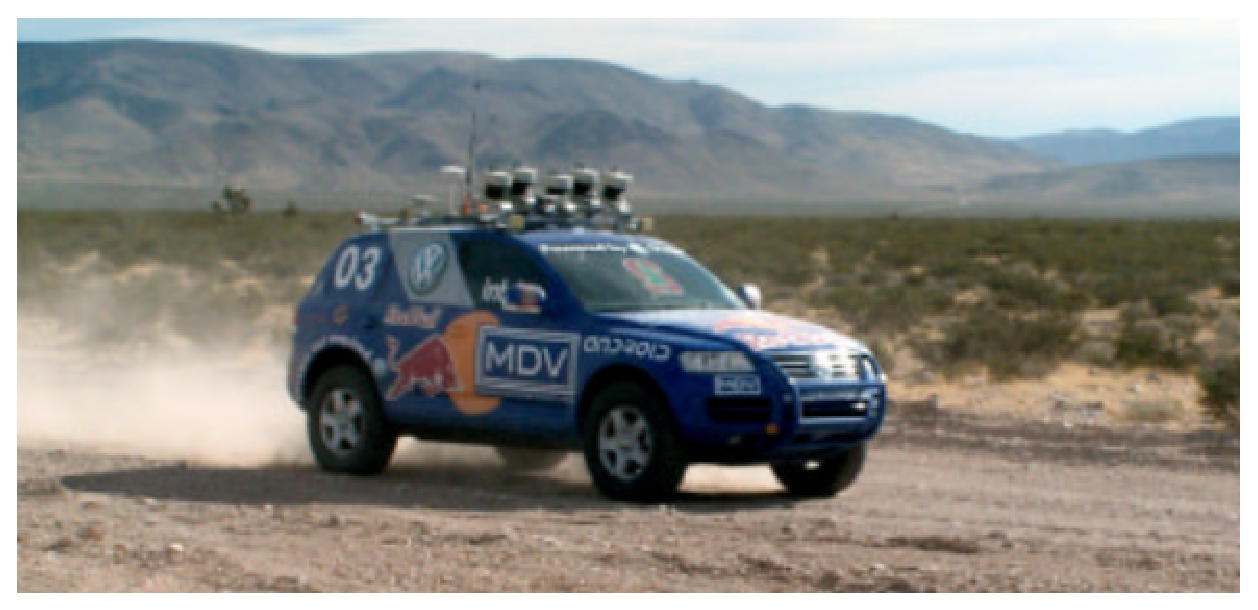
\includegraphics[height=3cm]{imgs/Stanley.eps}
		}
		\subfloat[\label{subfig:boss}]{%
			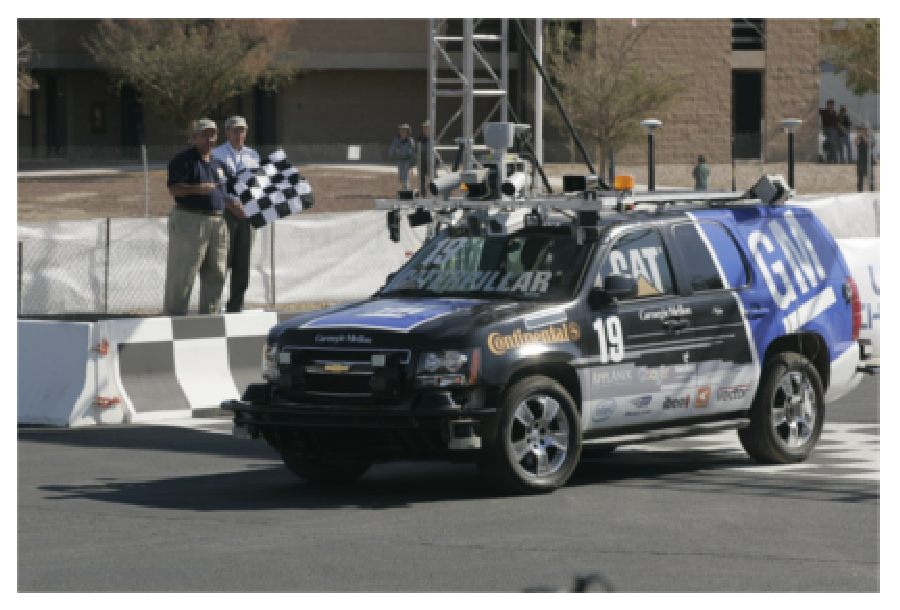
\includegraphics[height=3cm]{imgs/Boss_DARPA_urban_challenge.eps}
		}
	}
	\caption{The winning robots from the 2005 \ac{DARPA} Grand Challenge and 2007 Urban Challenge.~\protect\subref{subfig:stanley} shows Stanford's Stanley at the 2005 \ac{DARPA} Grand Challenge (Image from \cite{Thrun2006}),~\protect\subref{subfig:boss} shows Carnegie Mellon's BOSS at the 2007 \ac{DARPA} Urban Challenge (Image from \cite{Urmson.2008}).}\label{fig:darpa_chal}
\end{figure}

The technology developed for the \ac{DARPA} challenges formed the basis for commercial \ac{ADAS}, which have seen rapid progress since then and gradually made their way into series-production vehicles.
There exists a large variety of commercial systems, like e.g. \ac{ACC} or intelligent parking assistance systems, modern vehicles are already equipped with.
These systems have the potential to increase comfort and safety in road traffic and, in the long run enable fully autonomous driving (cf. Level \num{5}  in Table \ref{tab:autonomy_levels}).
On the other hand, many research teams and initiatives were spawned or inspired from these competitions and continued their research work after the \ac{DARPA} Challenges.
Many researchers involved in the winning teams continued their research within Google's self-driving car project, which started in 2009 and evolved into the Spin-Off company Waymo \cite{Waymo} in 2016.
Another research team continuing their efforts after the \ac{DARPA} challenges is the Annieway team \cite{Annieway}.
One of their major contributions is the release and maintenance of the KITTI vision benchmark suite \cite{Geiger2013a}, a publicly available data set containing data from various test drives in the city of Karlsruhe, rural areas as well as highways focusing on providing real world data for vision tasks like stereo, optical flow and 3D object detection and tracking.

The main research goal after the \ac{DARPA} Challenges was to develop automated driving with off-the-shelf sensors.
In \cite{Furgale2013}, the authors present a valet-parking approach for electrified vehicles using close-to-market sensors only.
\cite{Lundgren2014} shows an approach to vehicle self-localization using off-the-shelf sensors in combination with a detailed map.
In \cite{Aeberhard2015}, results from extensive testing of automated vehicles using mainly off-the-shelf sensors in highway scenarios are presented.
The sensors used are \ac{RADAR} sensors for long-range detection, \acf{US} sensors for redundant, close-range detection, a \ac{SensGPS} for vehicle-self localization as well as a front-facing mono camera, which are all available and integrated in series-production vehicles.
The only exception are 2D \ac{LIDAR} sensors, which are needed for high-resolution surround view.

\subsection{Knowledge Representation}
\label{subsec:knowledge_representation}

As a consequence of increasing complexity of \ac{ADAS} applications, the number of sensors mounted in modern vehicles has grown in recent years and is likely to grow even further in the near future to cover the vehicle's surrounding as completely as possible.
Another factor that leads to an increasing number of sensors in automotive context are safety considerations, which demand for redundancy in the overall setup to ensure functionality even in case of failure of one sensor.
Therefore, automated vehicles need to have a way to combine information from multiple sensor sources.
In the literature, the distinction between different approaches is typically made based on the level at which sensory data is combined \cite{Elfring2016}.
The two main classes of approaches are mostly referred to as \emph{low-level} and \emph{high-level} sensor fusion.
By \emph{low-level} sensor fusion, we mean that raw, previously unprocessed sensor measurements are combined in a coherent representation fur further processing.
In contrast, the goal of \emph{high-level} sensor fusion is to combine preprocessed tracks or features, that have been extracted from raw sensor measurements by each individual (smart) sensor unit.

\subsubsection{Representations for low-level sensor fusion}

\begin{figure*}[t!]
	\centering
	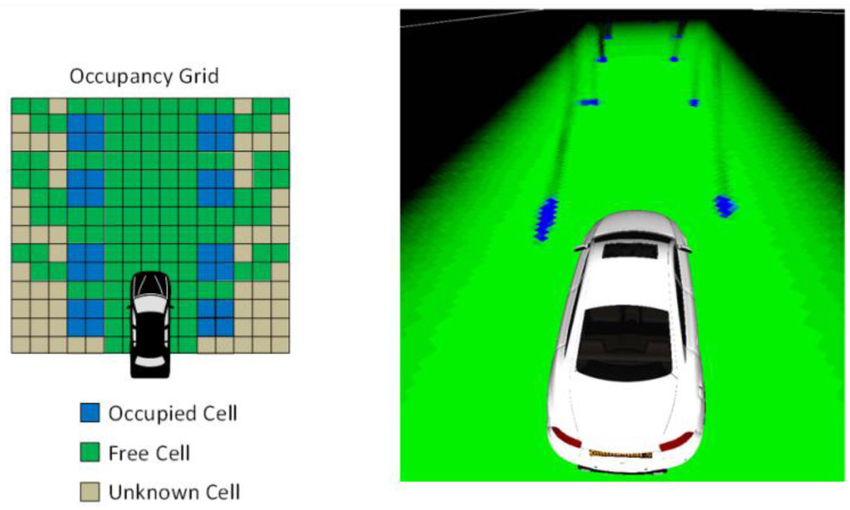
\includegraphics[width=0.95\textwidth]{imgs/occupancy_grid_principle.png}
    \caption{Occupancy-grid visualization for low-level sensor fusion. The left part depicts the principle of occupancy-grids, whereas the right part shows a real world example. Image source \cite{Hohm2014}}
	\label{fig:occupancy-grid}
\end{figure*}

One of the most widely used representations to combine low-level sensory data in robotics is an occupancy-grid map.
This representation is widely used for mobile robot localization \cite{Thrun2005}, but there is also a substantial amount of research regarding occupancy-grids regarding automotive environment modeling  \cite{Tanzmeister2014, Steyer2018}.
The left part of fig.~\ref{fig:occupancy-grid} visualizes the principles of occupancy-grids, whereas the right part shows a real world example from automotive context.
An occupancy-grid divides the represented space in discrete cells, which can take on different occupancy values (e.g., free, occupied or unknown).
The basic assumptions for this representation are that the world is static at each time step and that each cell can have exactly one occupancy value, i.e., one cell is for example completely occupied or completely free.
Therefore, an occupancy-grid is a well-suited representation for range sensors such as \ac{RADAR} or \ac{LIDAR} sensors.
While static occupancy-grid maps are mainly used for localization and \ac{SLAM} applications, there are also approaches to estimate dynamic parameters such as orientation and velocity within the grid to model dynamic environments \cite{Tanzmeister2014}.
The incoming raw sensory data is typically combined through some sort of probabilistic (Bayesian) filter algorithm such as Kalman- \cite{Kalman1960} or particle-filters \cite{Gordon1993}.
One of the main advantages of such a representation is that it is able to incorporate raw, unprocessed sensory data and that the discretization steps as well as the size of the cells can be chosen as fine-grained as the application demands.
Furthermore, it is a natural and precise way to model and represent the free, traversable space around the robot.
On the other hand, occupancy-grids have rather high requirements regarding memory and computational resources.
Additionally, the representation contains no information about type or properties of the obstacles that lead to cells being occupied.
Finally, in contrast to higher-level, more abstract representations, it can be more complex to incorporate sensor modalities other than range finders such as vision sensors.

\subsubsection{Representations for high-level sensor fusion}

In contrast to the low-level sensor fusion representation approaches described previously, high-level sensor fusion typically refers to sensory data being fused, that has already been preprocessed though some sort of temporal filtering.
This usually happens at \emph{tracked objects} level, i.e., object lists provided by individual sensor units each applying their own temporal filtering or tracking based on the data they receive.
To actually combine this sort of information, Bayesian filter approaches similar to the ones mentioned previously could be applied. 
However, such filters assume uncorrelated data and thus may deliver overconfident or diverging estimates since objects provided by different filters coming from several sensor sources are in fact correlated due to phenomena such as shared modeling assumptions, common noise acting on the objects being tracked or measurements arriving out of sequence.
Therefore, more advanced track-to-track fusion algorithms need to be used for high-level sensor fusion \cite{Tian2010, Aeberhard2012}.
These methods typically differ regarding the amount of knowledge they assume to be known about the correlations between the tracks.

The main advantages of high-level sensor fusion are that the amount of transferred data is lower compared to low-level fusion due to the hierarchical structure of the estimation framework.
Furthermore, as many sensors already employ on-board processing and provide data only at tracked object level, implementation of high-level fusion often does not require in-depth knowledge of the sensor characteristics.
This gives a more abstract interface and allows for easier replacement of individual sensor units in case the overall setup changes.
On the other hand, high-level fusion ignores potentially useful information, as it might be discarded at sensor level before the fusion is performed.
In summary, high-level sensor fusion is arguably the most popular and frequently used approach for combining information from different sensor sources in automated driving.
The objects are typically represented as "point objects" using a unique identifier and a state vector for dynamic information such as position, velocity and acceleration.
For certain application types, additional information such as the objects' size, shape and type need to be known (e.g., pedestrians have different dimensions and motion characteristics compared to trucks or vehicles).
For other objects of interest (e.g., traffic signs or traffic lights), color and shape information might be important.
While this type of representation is compact and abstract enough and thus well-suited for high-level fusion, the content and thus the represented values might vary depending on the sensor providing the information.
Therefore, achieving a unified representation across different sensor modalities can become a challenging problem.

\subsubsection{Other representations}

Representation approaches other than the aforementioned ones are rather rarely used in an automotive context.
Although semantic and structured information will grow more important with the advent of numerous and increasingly complex machine learning driven assistant systems, representations that are able to capture and manipulate such information are still hardly used in vehicle context.
One example of an abstract vector representation in an automotive context is Drive2Vec \cite{Hallac2018}, an unsupervised embedding of low-level sensory data to a vector, which is subsequently used to make predictions about the vehicle's state.
Similar to word embedding approaches, Drive2Vec learns an embedding from a high-dimension vector space (i.e., language or in this case several sensor streams) to a vector representation of comparably low dimension (representational space).
Another example of an alternative knowledge representation approach is the work presented in \cite{Yamazaki2016}, where the authors use symbolization, a language modeling technique, to obtain semantic descriptions of driving scenes.

\subsection{Driving Context Classification}%
\label{subsec:driving_context_classification}

Classification of the current driving context, i.e., if the vehicle is currently driving on a highway or in an urban area, has been investigated mainly in the earlier days of \ac{ADAS} research before digital maps were available at a large scale, which could be used in combination with the vehicle's current position measured using \ac{SensGPS} to detect the driving context.
However, inferring contextual information from on-board sensory data is appealing as either a fallback option in situations when \ac{SensGPS} is not available of if keeping an updated map with driving context information is not feasible.
Another simple approach is to classify the current driving context based on a set of conditional, logical rules using if-else statements such as "if the current velocity is greater than \SI{100}{\kilo\meter\per\hour}, then the current context is \emph{highway}".
However, this simple approach suffers from poor scaling and the difficulty to formulate exact definitions of all possible target categories in advance.
Improving on a logical rule set, the approach proposed in \cite{Hauptmann1996} employs a combination of a fuzzy-logic system based on the ego-vehicle's dynamics such as velocity, active gear and acceleration and a data-driven feed-forward neural network, which additional uses a front-facing camera.
In \cite{Engstrom2001}, the authors apply statistical pattern recognition and a simple feed-forward neural network using solely the ego-vehicle's dynamics to classify four different different driving context categories.
More modern approaches tend to focus more on the classification and analysis of particular traffic situations \cite{Hermann2008} or driving events \cite{Dagostino2013}, which can then be put in relation to the driver's behavior.

\subsection{Object Detection and Classification}
\label{subsec:obj_detect}

\begin{figure}[t!]
    \centering
    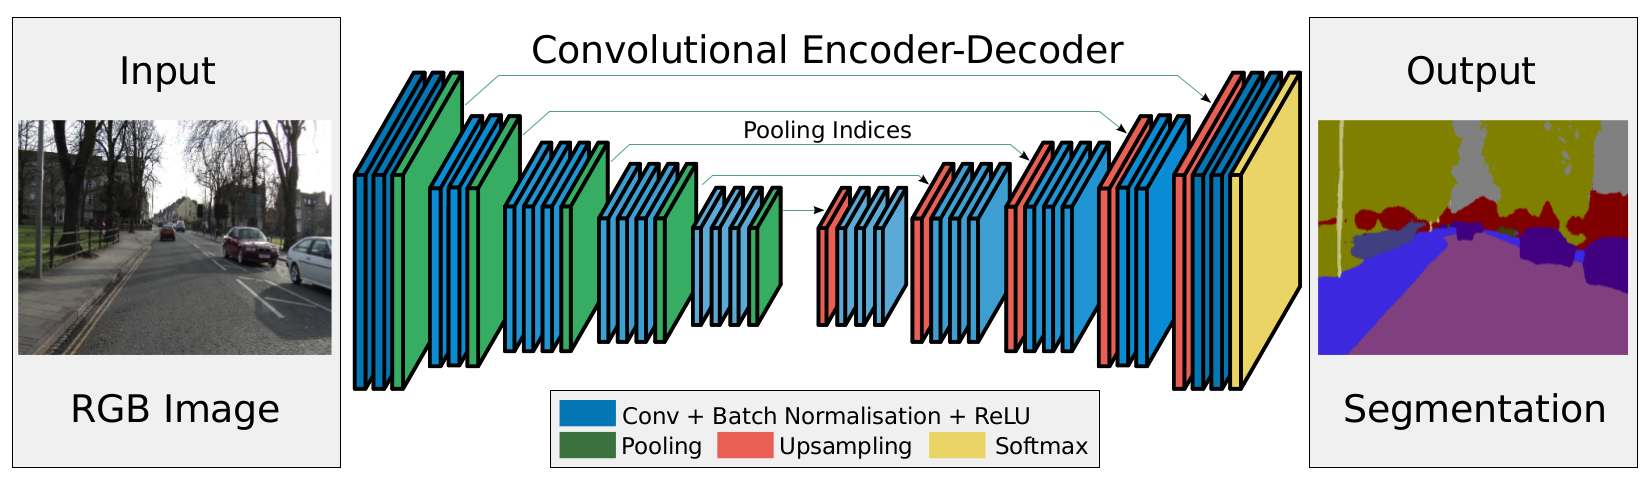
\includegraphics[width=0.95\linewidth]{imgs/segnet.png}
    \caption{Illustration of the SegNet \ac{FCN} architecture for semantic segmentation of an image visualizing the input data as well as the output of the network with pixel-wise labels indicating class membership. Image source \cite{Badrinarayanan2015}}
    \label{fig:segnet_achitecture}
\end{figure}
Detecting objects in the vehicle's surroundings and classifying their type is a central research problem in automated driving and more generally, in \ac{AI}.
Knowledge about type, position and behavior of other traffic participants as well as road lane topology is a crucial component for safe automated driving.
The algorithmic choice for detecting dynamic objects depends heavily on the sensor modality used.
If \ac{LIDAR} sensors are used, typically model-based approaches involving the object's geometry and dynamics are employed \cite{Petrovskaya2009a, Petrovskaya2009, Darms2008}.
Classic computer vision approaches employ probabilistic methods combined with information about context, scale or shapes detected using engineered features such as part-based models or \ac{HOG} features to identify cars \cite{Held2012}, traffic signs \cite{Li2015} or the road topology \cite{Alvarez2011, Beyeler2014}.
Such methods however have been drastically outperformed in recent years through sophisticated \acp{DNN} architectures such as \acp{CNN} achieving remarkable results on tasks like traffic sign detection \cite{Ciresan2012, Sermanet2011} achieving partly super-human performance \cite{Stallkamp2012}.
Subsequently, \acp{DNN} have been used to segment the road, or more generally, the traversable space \cite{Mohan2014, Bittel2015} or for semantic segmentation of the complete image, i.e., labeling each pixel in the image with the object class it belongs to (cf.\ fig.~\ref{fig:segnet_achitecture}), using \acp{FCN} \cite{Badrinarayanan2015, Long2015, Chen2018}.
The approach proposed in \cite{Li2017} deals with the special case of detecting vulnerable road users, i.e., pedestrians and bicyclists, by incorporating a \ac{CNN} variant for classification and localization.
In \cite{Huval2015}, the authors evaluate general applicability and usability of \acp{CNN} for lane and vehicle detection when deployed on a real-time critic system concluding that powerful \acp{GPU} enable real-time capabilities of such approaches.
An overview over recent approaches to tackle object detection and semantic segmentation using \acp{DNN} in an automotive context can be found in \cite{Feng2019}, while \cite{Janai2017} gives a more general overview of computer vision for automated vehicles.

\subsection{Trajectory Prediction}%
\label{subsec:trajectory_prediction}

\begin{figure*}[t!]
	\centering
	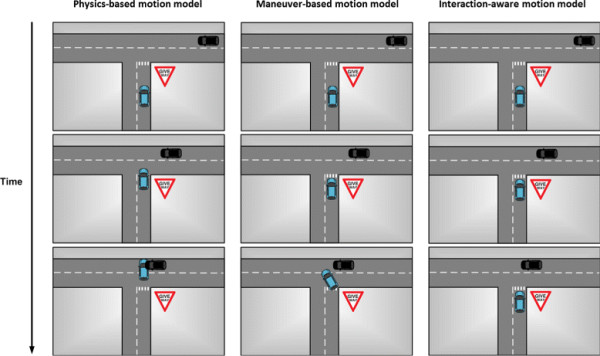
\includegraphics[width=0.95\textwidth]{imgs/examples_motion_prediction_models.jpg}
	\caption{Examples visualizing different modeling approaches for motion prediction in automotive context, Image source \cite{Lefevre2014}}
	\label{fig:examples_motion_prediction_types}
\end{figure*}
Predicting future behavior and positions of other traffic participants from observations is essential for collision avoidance and thus safe motion planning, and needs to be solved by human drivers and automated vehicles alike to reach their desired goal.
However, future positions of vehicles not only depend on each vehicle's own past positions and dynamics like  velocity and acceleration, but also on the behavior of the other traffic participants in the vehicle's surroundings.
Motion prediction for intelligent vehicles in general has seen extensive research in recent years, as it is a cornerstone for collision-free automated driving. \cite{Lefevre2014} classify such prediction approaches into three categories, namely \emph{physics-based}, \emph{maneuver-based} and \emph{interaction-aware}, depending on their level of abstraction.
Figure~\ref{fig:examples_motion_prediction_types} illustrates the differences between the three families of approaches: the \emph{physics-based} approach assumes a constant velocity of both vehicles, whereas the \emph{maneuver-based} approach assumes that the blue car turns left while the black car goes straight.
Finally the \emph{interaction-aware} approach assumes similar motions as the \emph{maneuver-based} approach whereas the motion of each vehicle is constrained by the traffic rules as well as the relative behavior of the other car.

\emph{Physics-based} approaches represent vehicles as dynamic entities, which obey the laws of physics.
To predict future motion, such approaches employ dynamic and kinematic models linking contrl inputs, car properties and external condition to the evolution of the state of the vehicle.
Hence, such approaches are well-suited for short term trajectory prediction but suffer from instabilities when predicting longer time-windows into the future and are unable to account for any change in vehicle motion caused by a particular maneuver (e.g., slowing down or performing a turn). 
\emph{Maneuver-based} approaches are more advanced assuming the vehicle motion is a series  of maneuvers, which are performed independently from the other traffic participants.
Such approaches rely on early detection of the maneuver the driver intends to perform, which is then assumed to match the future behavior of the vehicle.
If the identification of the maneuver was correct, these approaches allow for more accurate long term predictions compared to purely physics-based approaches.
However, they ignore potential interconnections in the motion between several traffic participants, which, in practice, share the road and the motion of one vehicle will influence the motion of other vehicle in its surroundings.

\begin{figure}[t!]
    \centering
    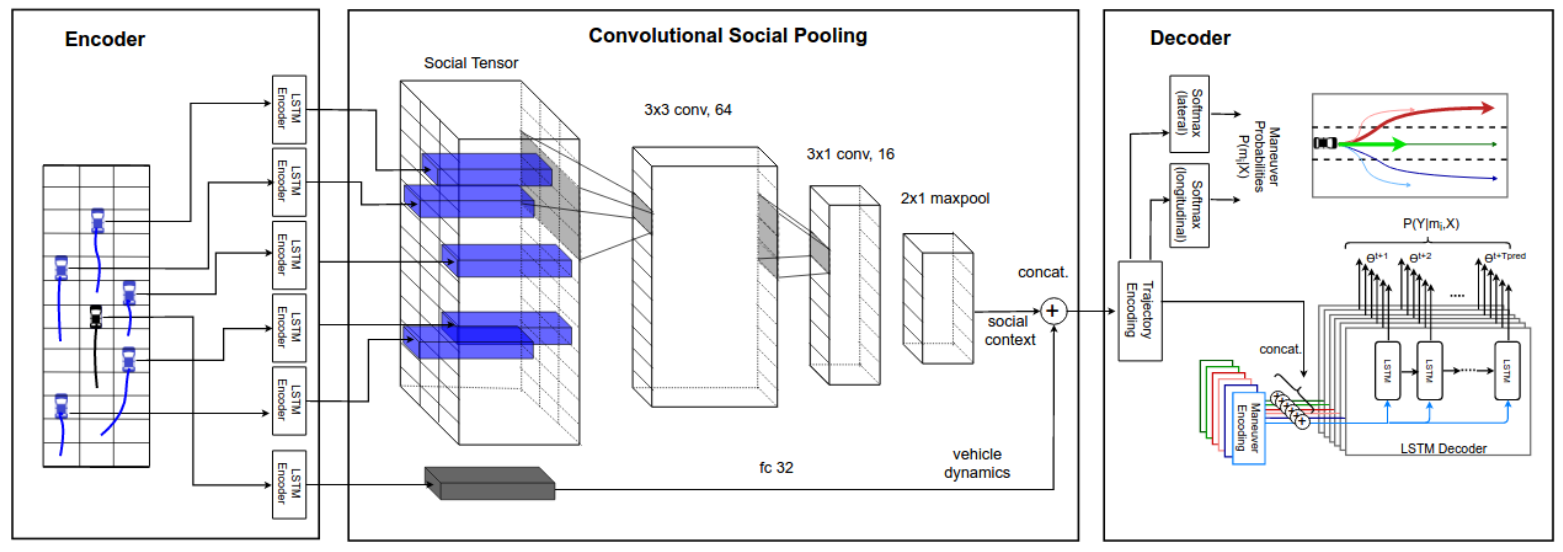
\includegraphics[width=0.95\linewidth]{imgs/deo_lstm_prediction_arch.png}
    \caption{Visualization of one state-of-the-art \ac{LSTM}-based architecture for vehicle trajectory prediction combining social pooling to account for the influence of other vehicles on the target vehicle with a maneuver-based prediction module. Image source \cite{Deo2018a}.}
    \label{fig:deo_lstm_prediction_arch}
\end{figure}

There exist a growing number of different \emph{interaction-aware} approaches to account for those dependencies and mutual influences between traffic participants or, more generally, agents in the scene.
Probabilistic models like cost maps \cite{Bahram2016} account for physical constraints on the movements of the other vehicles.
Classification approaches categorize and represent scenes in a hierarchy \cite{Bonnin2012} based on the most generic ones to predict behavior for a variety of different situations.
Data-driven approaches to behavior prediction mainly rely on \ac{LSTM} neural network architectures \cite{Hochreiter1997}, which have proven to be a powerful tool for sequential data analysis.
\cite{Alahi2016} model interactions in the learning network architecture by introducing so-called social-pooling layers to connect several \acp{LSTM} each predicting one agent at a time.
The authors in \cite{Altche2018} use a \ac{LSTM} network and account for interactions by including distances between the target vehicle and other agents directly in the training data.
A similar approach is proposed in \cite{Deo2018}, but it combines \ac{LSTM} networks with an additional maneuver classification network to predict future vehicle motion.
In \cite{Deo2018a}, the authors adapted the combination of several \ac{LSTM} networks to encode vehicle trajectories, (convolutional) social-pooling layers to account for interactions between the vehicles, and a maneuver-based \ac{LSTM} decoder to predict vehicle trajectories in highway situations (see figure~\ref{fig:deo_lstm_prediction_arch}).
\ac{LSTM}-models are currently considered the most successful approaches and therefore the state-of-the-art regarding trajectory prediction.
One issue with data-driven approaches to behavior prediction accounting for relations between agents is that the number of other vehicles is variable.
If information about vehicles other than the target are encapsulated in the input of the neural network, typically a specific number of other vehicles of interest are manually chosen a priori to avoid this issue \cite{Altche2018, Deo2018}.
If the information about other vehicles is encapsulated in the network architecture, it might be necessary to train several networks depending on the situation at hand.

\subsection{Online Learning}%
\label{subsec:online_learning}

Common to all approaches mentioned in section~\ref{subsec:trajectory_prediction} is the fact, that the models are trained offline on batched data and remain unchanged during deployment.
In contrast, incremental or online learning approaches, which attempt to tackle learning tasks by processing sequential data one at a time, gained growing interest as an attractive alternative to update learning models during deployment.
This approach is particularly interesting in the context of big data and in situations, where the system needs to learn from continuously incoming data streams and a complete data set during offline training is not available.
There exists an increasing number of online learning approaches in several problem domains (see \cite{Losing2018}, \cite{Gomes2017} or \cite{Hoi2018} for a comprehensive overview of the field).
However, such models adapting their (neural) weights at run time through online learning are rather rarely investigated in automotive context due to safety considerations, issues with convergences time as well as the lack of proofs/guarantees that the models converge at all.
The model presented in \cite{Maye2011} uses self-supervised online learning to recognize, classify and add new maneuvers of the ego-vehicle at run time.
The approach employed in \cite{Graf2014} uses case-based reasoning to learn to predict driving behavior for specific driving situations, namely intersection scenarios.
In \cite{Losing2017}, the authors employ incremental learning to personalize maneuver prediction at intersections.
An alternative approach to combining several weak learning models such as stumps or smoothing splines through an averaging scheme is boosting \cite{Taieb2014}, which offers superior performance over the individual learners.
An online learning approach based on \acp{SNN} has been shown to be successful in similar domains such as adaptive robot arm control \cite{DeWolf2016}, but has not been applied yet in an automotive application such as trajectory prediction.

\subsection{Data sets}%
\label{subsec:data_sets}

With the advent and success of sophisticated \ac{DNN} architectures and their success in several domains related to automated driving such as object detection (see section~\ref{subsec:obj_detect}) and behavior prediction (see section~\ref{subsec:trajectory_prediction}), the demand for large-scale data sets for training such networks grew significantly in recent years.
Furthermore, there is an interest in publicly available data sets which not only enable competition between researchers but also allow for transparent benchmarking of approaches against each other.
Data sets for image classification such as the \ac{MNIST} data set for hand-written digits \cite{LeCun1998} , the \ac{GTSRB} for traffic sign recognition \cite{Stallkamp2012} and the ImageNet data set \cite{Deng2009} provided researchers with large amounts of labeled image data facilitating significant progress in this research field.

One of the first data sets being made publicly available on a larger scale for research in an automotive context and encouraging competition is the KITTI vision benchmark suite \cite{Geiger2013a}, which was recorded using the Annieway vehicle prototype \cite{Annieway} in urban environments in the region of the German city Karlsruhe.
The KITTI data set offers raw sensory data for different sensor modalities such as \ac{LIDAR} and vision alongside ground truth labels and benchmarks for several tasks such as road detection, object detection, optical flow and tracking.
Another large-scale data set targeted at computer vision in an automotive context is the Cityscapes data set \cite{Cordts2016}. 
It provides high-definition images recorded from a driving vehicle with accurate pixel-wise labels for semantic segmentation.
Furthermore, the Cityscapes data set also contains labels for depth information obtained from stereo vision, which for instance allows to train neural networks to provide depth information based only on monocular input. 
A comparable data set for semantic image segmentation in a broader context (i.e., not restricted to an automotive context) is the 
\ac{COCO}  data set \cite{Lin2014}.
Furthermore, the \ac{COCO} data set is also provides ground truth captions for each images allowing to train neural networks translating visual input to language. 
Another more recent data set similar to the KITTI data set is the Apollo Scape data set \cite{Huang2018}, which is provided by the Chinese company Baidu and contains data and ground truth labels for several automotive applications such as scene parsing, lane segmentation, localization, tracking and trajectory prediction.
The \ac{NGSIM} US-101 data set \cite{NGSIM-US101} is a publicly available data set originally intended for driver behavior and traffic flow models \cite{He2017}, that has been used to train trajectory predictions models \cite{Altche2018, Deo2018} as well.
It was recorded on a segment of approximately \SI{640}{\meter} length with \num{6} lanes on the US-101 freeway in Los Angeles, California  using cameras observing freeway traffic from rooftops with trajectory-data being extracted later from the obtained video footage.

\section{Summary}
\label{sec:related_work_summary}

In this chapter, we have taken a round trip through several research areas related to the thesis at hand.
We visited the historical and current developments in the field of \ac{AI}, machine learning and neuromorphic engineering.
Especially the young and emerging research field of neuromorphic engineering shows promise to be an energy-efficient possibility for future applications with tight restrictions regarding their energy-budget and computational resources.
As a mobile application with a growing number of sensors and increasingly complex modules (often employing modern machine learning techniques) involved not only in autonomous navigation but also for interacting with the passengers inside and other traffic participants outside the car, intelligent vehicles in general offer promising application possibilities for the technology developed in this research area.
However, the computing hardware prototypes \cite{Furber2014, Akopyan2015, Davies2018} as well as the novel senor technologies \cite{Lichtsteiner2008} are not mature enough yet to either become commercial products or to be deployed in series-production vehicles.
Additionally, the principles of \acp{SNN} in combination with dedicated computing hardware show promise to be an energy-efficient algorithmic substrate to be applied in future automotive applications.
However, this algorithmic approach has only been investigated in rather simple robotic applications \cite{Conradt2014, Stewart2016, Galluppi2014} and, similar to the neuromorphic hardware, is not mature enough yet, especially for such safety-critical applications like automated driving.

Furthermore, we presented an overview of different architectures for cognitive modeling putting emphasis on vector-based representations such as the \ac{SPA} or, more generally, \acp{VSA}.
After showing alternative approaches such as symbolic and connectionist cognitive architectures, we also reviewed the most prominent applications of such architectures and the representations they employ.
We have seen, that there is a gap between architectures that are well-suited for modeling higher-level cognitive tasks and lower-level tasks closer to the dynamics of perception and action.
While the former is most successfully tackled with symbolic modeling architectures, the latter often demands for precise mathematical modeling for dealing with the complexity and dynamics of real-world physics.
Therefore, little attempts have been made to use cognitive modeling in real robotic systems and if, the investigated tasks are often simplified \cite{Neubert2016} and still far away from the demands imposed by complex systems like automated vehicles.
Although we do not attempt to close this gap in our proposed work, we show that structured vector representations are an interesting option for encode automotive scenes in an abstract, unified and sensor independent substrate.
Today's sensing and processing hardware is currently not intended to support such a representation.
However, the full strength of this approach can only unfold once it is possible to employ cognitive modeling and spiking neuron principles in the complete chain from sensing to behavior with dedicated hardware support.

Finally, we summarized the current state-of-the-art in several sub-domains of automated driving related to our work.
After a brief historical overview, we focused on reviewing the currently used approaches for representing knowledge in an automotive context.
As stated earlier, the techniques employed here use mainly Bayesian statistics and mathematical modeling to deal with the complexity of the real world.
Subsequently, we reviewed the state-of-the-art in several selected tasks from sub-domains related to automated driving.
These tasks mirror the application examples we have chosen as use-cases to investigate our approaches and will be revisited in subsequent chapters (see chapters~\ref{chap:driving_context_classification},~\ref{chap:behav_pred} and~\ref{chap:mix_online_learning}).

Admittedly, our work touches and incorporates prior work from very different research fields by developing an approach for representing automotive scenes in an abstract vector representation inspired by modern cognitive modeling approaches.
To the best of our knowledge, our work is the first to employ such a unified vector representation in an automotive context.
The only other work encapsulating vehicle data in a compact vector representation is \cite{Hallac2018}, whose approach uses sensory data at a far lower level (i.e., closer to the actual sensor data) than we do and targets different application scenarios.

In the next chapter, we give a detailed introduction to the mathematical theory behind \acp{VSA} in general and more specifically to the \ac{SPA} as well as to the principles of the \ac{NEF}.
Together with the review presented here, this  will form the theoretical basis for the remainder of the thesis.
